% Compile from journal_article/: pdflatex main; biber main; pdflatex main; pdflatex main
\documentclass[11pt,a4paper]{article}
\usepackage[utf8]{inputenc}
\usepackage[T1]{fontenc}
\usepackage[english]{babel}
\usepackage[margin=25mm]{geometry}
\usepackage{newtxtext,newtxmath}
\renewcommand{\ttdefault}{lmtt}
\usepackage{amsmath,mathtools}
\usepackage{graphicx,booktabs,ragged2e,etoolbox,placeins,needspace}
\usepackage{tabularray}
\UseTblrLibrary{booktabs,siunitx}
\usepackage[font=small,labelfont=bf,labelsep=period]{caption}
\usepackage{csquotes}
\usepackage[backend=biber,style=authoryear,maxcitenames=2,maxbibnames=99,doi=true,isbn=false,url=false]{biblatex}
\addbibresource{references.bib}
\usepackage[hidelinks]{hyperref}
\usepackage{microtype}
\SetTblrInner[booktabs]{width=\textwidth,row{1}={font=\bfseries},hline{1,Z}={0.8pt},hline{2}={0.4pt}}
\SetTblrStyle{remark-text}{font=\footnotesize}
\SetTblrStyle{remark-tag}{font=\footnotesize\itshape}
\newenvironment{tablenotes}[1][Note]{\par\medskip\begingroup\footnotesize\noindent\textit{#1:} }{\par\endgroup}
\newenvironment{figurenotes}[1][Note]{\par\medskip\begingroup\footnotesize\noindent\textit{#1:} }{\par\endgroup}
\newlength{\baselinedist}\setlength{\baselinedist}{\baselineskip}
\setlength{\emergencystretch}{2em}
\setcounter{topnumber}{3}\setcounter{totalnumber}{4}
\renewcommand{\topfraction}{.95}\renewcommand{\textfraction}{.05}
\renewcommand{\floatpagefraction}{.75}
\raggedbottom

\title{High-Dimensional Instrumental Variable Quantile Regression under Weak Instruments: A Monte Carlo Study}
% Shared affiliation and individual contact details; no corresponding author.
\author{\begin{minipage}{\dimexpr\textwidth-2\tabcolsep\relax}\centering
\normalsize OLIMJON UMIDJON UGLI UMURZOKOV\textsuperscript{a}\\
\small ORCID: \href{https://orcid.org/0009-0008-0090-7100}{0009-0008-0090-7100}\\
Email: \href{mailto:olimumurzokov022@gmail.com}{olimumurzokov022@gmail.com}\\[0.7em]
\normalsize UMIDJON UMIRZAKOVICH KOSTAEV\textsuperscript\\
\small ORCID: \href{https://orcid.org/0009-0000-0205-5142}{0009-0000-0205-5142}\\
Email: \href{mailto:umidjonkostaev2025@gmail.com}{umidjonkostaev2025@gmail.com}\\[0.7em]
\end{minipage}}
\date{}
\hypersetup{pdftitle={High-Dimensional IVQR under Weak Instruments},pdfauthor={UMIDJON UMIRZAKOVICH KOSTAEV; OLIMJON UMIDJON UGLI UMURZOKOV}}
\begin{document}
\maketitle
\begin{abstract}
We examine how weakening instrument relevance affects high-dimensional instrumental variable quantile regression (IVQR). A controlled extension of the Monte Carlo design of Chen, Huang, and Tien (2021) reduces the excluded signal while adding independent noise to preserve the marginal treatment distribution and the relationship generating endogeneity. Oracle-GMM, Full-GMM, and double/debiased machine learning IVQR (DML-IVQR) are compared across four relevance settings, five quantiles, and sample sizes of 500 and 1000, using 500 replications per design. As relevance declines, point-estimation errors increase, finite-domain accepted sets expand, and power generally falls, including for the oracle benchmark. Coverage can approach its nominal level while inference becomes uninformative; substantial undercoverage also occurs in several strong-relevance cells. DML-IVQR often improves point accuracy relative to Full-GMM, with exceptions. The evidence concerns a preserved executable implementation with an asymptotic chi-square cutoff, implementation-specific residualization and density proxies, and no cross-fitting. Orthogonalization and regularized nuisance estimation can mitigate high-dimensional estimation difficulties, but cannot replace identifying information lost as instrument relevance deteriorates.
\end{abstract}
\noindent\textbf{Keywords:} instrumental variable quantile regression; double machine learning; weak instruments; Monte Carlo simulation; confidence-set informativeness
\section{Introduction}
Heterogeneous treatment effects motivate analysis across the potential-outcome distribution, but endogenous treatment prevents conventional quantile regression from recovering structural effects. Instrumental variable quantile regression (IVQR) combines excluded instruments with structural-rank restrictions to address this problem \parencite{koenker_bassett_1978,chernozhukov_hansen_2005}. In applications with many controls, nuisance estimation introduces an additional difficulty. Regularization and Neyman-orthogonal moments can reduce its impact on inference, but neither creates identifying information when instruments explain little treatment variation.

The IVQR literature distinguishes moment validity from identification and informative inference \parencite{chernozhukov_hansen_wuthrich_2017}. Inverse quantile regression provides practical estimation under regular identification \parencite{chernozhukov_hansen_2006}; candidate-specific test inversion accommodates weak identification under its maintained regularity conditions \parencite{chernozhukov_hansen_2008}. Its accepted regions can nevertheless be wide or disconnected. The finite-sample conditional procedure of \textcite{chernozhukov_hansen_jansson_2009} is a separate inferential construction. Related developments in the broader IV literature include the direct structural tests of \textcite{anderson_rubin_1949}, weak-IV approximations \parencite{staiger_stock_1997}, weak-identification-robust GMM \parencite{stock_wright_2000}, and pivotal and conditional likelihood-ratio procedures \parencite{kleibergen_2002,moreira_2003}. \textcite{andrews_stock_sun_2019} review their implications. Conventional first-stage diagnostics describe relevance, but do not provide universal quantile-specific IVQR identification thresholds.

High-dimensional regularization addresses a different source of difficulty. \textcite{belloni_chernozhukov_2011} develop penalized quantile regression and pivotal penalty calibration; \textcite{belloni_chernozhukov_kato_2019} establish orthogonal-score inference in approximately sparse quantile models. Double/debiased machine learning (DML) uses Neyman orthogonality to reduce first-order sensitivity to sufficiently small nuisance errors \parencite{chernozhukov_et_al_2018}. Cross-fitting is a distinct device for separating nuisance estimation from score evaluation. \textcite{chen_huang_tien_2021} combine regularized nuisance estimation and an orthogonal IVQR score, comparing Oracle-GMM, Full-GMM, and DML-IVQR in a high-dimensional Monte Carlo design. Further approaches address endogenous binary treatment \parencite{wuthrich_2019} and orthogonal moments for nonparametric IVQR with high-dimensional covariates \parencite{jin_sun_2025}.

The high-dimensional simulation in \textcite{chen_huang_tien_2021} holds instrument relevance fixed. We ask how progressively weakening that relevance changes point accuracy, coverage, power, and confidence-set informativeness across quantiles. Our contribution is a controlled Monte Carlo extension of their design and preserved executable procedures. A relevance parameter scales the excluded signal, while compensating independent noise preserves the treatment distribution and its joint distribution with the outcome disturbance. The extension introduces neither a new estimator nor a new inference theory.

The experiment compares three complete implementations on common samples. Oracle-GMM knows the designated relevant controls; Full-GMM uses all controls without regularization; DML-IVQR regularizes nuisance estimation. As relevance falls, all three lose point accuracy and numerical localization, while power generally declines. DML-IVQR usually improves point accuracy relative to Full-GMM, with exceptions. Coverage can approach 95\% as tests lose discrimination, and several strong-relevance cells exhibit substantial undercoverage. The implementation differences, non-finite population density weight, and asymptotic reference distribution qualify interpretation throughout. These results separate the benefits of nuisance estimation from the information required to distinguish competing structural effects.

\section{Econometric Framework}
\label{sec:framework}
\subsection{Structural moments and orthogonalization}
Let $Y_i$ be the outcome, $D_i$ endogenous treatment, $X_i$ controls, and $Z_i\in\mathbb R^{d_z}$ instruments. Under the structural-rank assumptions of \textcite{chernozhukov_hansen_2005}, the monotone structural quantile function has the representation
\begin{equation}
    Y_i = q(U_i,D_i,X_i),
    \qquad
    U_i \mid X_i,Z_i \sim \operatorname{Uniform}(0,1),
    \label{eq:structural-ivqr}
\end{equation}

\begin{equation}
    q(\tau,D_i,X_i)
    = c_0(\tau)
      + D_i^{\prime}\alpha_0(\tau)
      + X_i^{\prime}\beta_0(\tau).
    \label{eq:linear-structural-quantile}
\end{equation}
The treatment coefficient $\alpha_0(\tau)$ is the target. The intercept and control coefficients are nuisances. Rank similarity permits treatment-state-specific ranks with the same relevant conditional distribution; rank invariance is the stronger common-rank case. The structural quantile at fixed treatment generally differs from the observational quantile conditional on endogenous treatment. Monotonicity and conditional rank uniformity imply
\begin{equation}
    \operatorname{E}\!\left[
        \tau
        - \mathbf{1}\!\left\{
            Y_i \leq c_0(\tau)
            + D_i^{\prime}\alpha_0(\tau)
            + X_i^{\prime}\beta_0(\tau)
        \right\}
        \mathrel{\big|} X_i,Z_i
    \right]
    = 0.
    \label{eq:ivqr-conditional-moment}
\end{equation}
Instrument validity supports this restriction; identification additionally requires variation that distinguishes alternative treatment coefficients.

For candidate $a$, define $\widetilde X_i=(1,X_i')'$, $\rho_\tau(v)=v[\tau-\mathbf1\{v<0\}]$, and the population nuisance profile
\begin{equation}
    \begin{pmatrix}
        c(a)\\
        \beta(a)
    \end{pmatrix}
    = \operatorname*{arg\,min}_{c,b}
      \operatorname{E}\!\left[
          \rho_{\tau}\!\left(Y_i-D_i^{\prime}a-c-X_i^{\prime}b\right)
      \right].
    \label{eq:profile-beta}
\end{equation}

\begin{equation}
    \epsilon_i(a)
    =Y_i-D_i^{\prime}a-c(a)-X_i^{\prime}\beta(a).
    \label{eq:profile-residual}
\end{equation}

\begin{equation}
    \begin{aligned}
        M(a)
        &=\operatorname{E}\!\left[
            Z_i\widetilde X_i^{\prime}f_{\epsilon(a)}(0\mid X_i,Z_i)
        \right],
        & M(a)&\in\mathbb{R}^{d_z\times(p+1)},\\
        J(a)
        &=\operatorname{E}\!\left[
            \widetilde X_i\widetilde X_i^{\prime}f_{\epsilon(a)}(0\mid X_i,Z_i)
        \right],
        & J(a)&\in\mathbb{R}^{(p+1)\times(p+1)}.
    \end{aligned}
    \label{eq:profile-MJ}
\end{equation}

\begin{equation}
    \delta(a)=M(a)J(a)^{-1},
    \qquad
    \delta(a)\in\mathbb{R}^{d_z\times(p+1)},
    \label{eq:profile-delta}
\end{equation}

\begin{equation}
    \Psi_i(a)
    =Z_i-\delta(a)\widetilde X_i
    =Z_i-d_0(a)-\Gamma(a)X_i.
    \label{eq:profile-residualized-instrument}
\end{equation}
Here $f_{\epsilon(a)}(0\mid X_i,Z_i)$ is the conditional residual density at zero. With $\eta=(c,\beta',\operatorname{vec}(\delta)')'$, let $\eta(a)$ collect the candidate-specific profile and $\eta_0=\eta(\alpha_0(\tau))$. The theoretical score is
\begin{equation}
    \begin{aligned}
        g_{\tau}(W_i;a,\eta)
        &=
        \left[
            \tau-\mathbf{1}\!\left\{
                Y_i\leq D_i^{\prime}a+c+X_i^{\prime}\beta
            \right\}
        \right]
        \left(Z_i-\delta\widetilde X_i\right),\\
        g_{\tau}(W_i;a,\eta(a))
        &=
        \left[
            \tau-\mathbf{1}\!\left\{
                Y_i\leq D_i^{\prime}a+c(a)+X_i^{\prime}\beta(a)
            \right\}
        \right]\Psi_i(a),
    \end{aligned}
    \label{eq:orthogonal-score}
\end{equation}

\begin{equation}
    \operatorname{E}\!\left[
        g_{\tau}\!\left(W_i;\alpha_0(\tau),\eta_0\right)
    \right]
    =0.
    \label{eq:orthogonal-score-moment}
\end{equation}

\begin{equation}
    \left.
    \partial_{\eta}
    \operatorname{E}\!\left[
        g_{\tau}\!\left(W_i;\alpha_0(\tau),\eta\right)
    \right]
    \right|_{\eta=\eta_0}
    =0.
    \label{eq:neyman-orthogonality}
\end{equation}
Under finite density-weighted moments, a nonsingular $J$, and the requisite differentiation conditions, the derivative in the intercept and slopes is $-[M_0-\delta_0J_0]=0$. The residualization derivative vanishes by the quantile moment. Appendix~\ref{app:score-algebra} gives the algebra. These are properties of the ideal construction under its conditions, rather than guarantees for every executable implementation.

This distinction is material for the present DGP. At truth, the outcome residual is $e_\tau=D(u-q_\tau)$, with $q_\tau=\Phi^{-1}(\tau)$ and $D=\Phi(T)$, $T=d^*(\kappa)$. Conditional on $u=q_\tau$, $X$, and observed $Z$, the variance of the normal index is $2.91-\kappa^2>1$ for every investigated setting. The density at zero contains a term proportional to $\operatorname E[1/\Phi(T)\mid u=q_\tau,X,Z]$, which is not finite. The experiment therefore does not establish the ideal density-weight regularity conditions or validate the associated asymptotic theory.

\subsection{Preserved estimators and inference}
\label{sec:implementation}
Oracle-GMM uses $X_1,\ldots,X_{10}$, the designated oracle set. Full-GMM uses all 100 controls. Both fit an unpenalized candidate-specific quantile regression with an intercept, then directly invert density-proxy-weighted control moment matrices without a residualization intercept. DML-IVQR fits quantile Lasso and regularized instrument regressions using all controls. Its Belloni--Chernozhukov pivotal penalty follows the executable route of \textcite{chen_huang_tien_2021}; their comparison with cross-validation motivates retaining this route.

The quantile-Lasso objective is an unscaled sum of check losses plus one half of the supplied coefficient-specific penalty vector times absolute coefficients, including the intercept. There is no post-Lasso refit. Instrument regressions use square-root-density-transformed instruments and controls with an ordinary unpenalized intercept. The score subtracts the retained intercept and original-control fitted slopes from the untransformed instrument. This intercept differs from the constant regressor in the ideal weighted projection. The fitted-normal proxy is evaluated at candidate residuals; the preserved R call \texttt{dnorm(e, mean(e), var(e))} supplies the residual variance where R interprets a standard deviation. It is not a direct estimate of the theoretical conditional density at zero.

Nuisances and scores use the same observations, with no sample splitting or cross-fitting. Fresh pivotal draws are generated at each penalty call, introducing algorithmic randomness across candidate evaluations. Appendix~\ref{app:reproducibility} records the penalty formulas, residualization rules, and environment details. The estimator comparison encompasses these implementation differences as well as regularization and nuisance dimension; it cannot isolate the effect of regularization alone.

For estimator $e$, let $\widehat g_{e,i}(a)$ be its score. The common criterion uses the uncentered score second moment:
\begin{equation}
    \widehat g_{e,n}(a)
    =
    \frac{1}{n}\sum_{i=1}^{n}\widehat g_{e,i}(a).
    \label{eq:sample-gmm-moment}
\end{equation}

\begin{equation}
    \widehat\Sigma_e(a)
    =
    \frac{1}{n}\sum_{i=1}^{n}
    \widehat g_{e,i}(a)\widehat g_{e,i}(a)^{\prime}.
    \label{eq:score-covariance}
\end{equation}

\begin{equation}
    W_{e,n}(a)
    =
    n\widehat g_{e,n}(a)^{\prime}
    \widehat\Sigma_e(a)^{-1}
    \widehat g_{e,n}(a).
    \label{eq:gmm-criterion}
\end{equation}

\begin{equation}
    \widehat\alpha_e(\tau)
    =
    \operatorname*{arg\,min}_{a\in\mathcal A}W_{e,n}(a).
    \label{eq:gmm-point-estimator}
\end{equation}
The Monte Carlo candidate set $\mathcal A$ is the fixed grid specified below; the first exact minimizer is retained, and an incomplete profile receives no point estimate. Direct inversions use neither a generalized inverse nor additional matrix regularization. Failures or non-finite statistics are recorded as numerical failures.

The procedures apply the asymptotic $\chi^2_{d_z}$ reference cutoff to each candidate statistic. At significance level $\gamma$, inversion gives
\begin{equation}
    \mathcal C_{e,1-\gamma}(\tau)
    =
    \left\{
        a\in\mathcal A:
        W_{e,n}(a)\leq c_{1-\gamma,d_z}
    \right\}.
    \label{eq:robust-confidence-region}
\end{equation}
Here $c_{1-\gamma,d_z}$ is the chi-square quantile, with $d_z=2$. The corresponding theoretical candidate tests can accommodate weak identification under their regularity conditions \parencite{chernozhukov_hansen_2008}; finite-sample calibration of these preserved implementations remains an empirical question. This construction differs from exact conditional finite-sample inference \parencite{chernozhukov_hansen_jansson_2009}. Weak-identification robustness does not ensure narrow sets or high power, and a finite numerical domain cannot establish global boundedness.

\section{Monte Carlo Design}
\label{chap:monte-carlo-design}
\subsection{Baseline and controlled relevance extension}
\label{sec:monte-carlo-design}
The baseline follows the executable high-dimensional design of \textcite{chen_huang_tien_2021}, with independent observations and 100 controls. The outcome and assignment disturbances satisfy
\begin{equation}
  \begin{pmatrix}
    u_i \\
    \epsilon_i
  \end{pmatrix}
  \sim
  \mathcal{N}\!\left(
    \begin{pmatrix} 0 \\ 0 \end{pmatrix},
    \begin{pmatrix} 1 & 0.3 \\ 0.3 & 1 \end{pmatrix}
  \right).
  \label{eq:dgp-disturbances}
\end{equation}

\begin{equation}
  x_{ji}\overset{\mathrm{ind}}{\sim}\mathcal{N}(0,1),
  \quad j=1,\ldots,100,
  \qquad
  z_{1i},z_{2i},v_{1i},v_{2i}
  \overset{\mathrm{ind}}{\sim}\mathcal{N}(0,1).
  \label{eq:dgp-primitives}
\end{equation}

\begin{equation}
  X_{ji}=\Phi(x_{ji}),
  \qquad j=1,\ldots,100,
  \label{eq:dgp-controls}
\end{equation}
The remaining primitives are mutually independent and independent of $(u_i,\epsilon_i)$. The controls $X_{ji}=\Phi(x_{ji})$ are independent Uniform$(0,1)$ variables. The observed instruments are
\begin{equation}
  Z_{1i}=z_{1i}+v_{1i}+X_{2i}+X_{3i}+X_{4i},
  \label{eq:dgp-instrument1}
\end{equation}

\begin{equation}
  Z_{2i}=z_{2i}+v_{2i}+X_{7i}+X_{8i}+X_{9i}+X_{10i}.
  \label{eq:dgp-instrument2}
\end{equation}
The released code uses transformed $X$ controls in these equations, although the source paper displays corresponding terms as lowercase $x$. We retain the executable construction. The baseline treatment and outcome are
\begin{equation}
  D_i=\Phi(z_{1i}+z_{2i}+\epsilon_i).
  \label{eq:dgp-treatment-baseline}
\end{equation}

\begin{equation}
  Y_i=1+D_i+5\sum_{j=1}^{7}X_{ji}+D_i u_i.
  \label{eq:dgp-outcome}
\end{equation}
The correlation of $u_i$ with $\epsilon_i$ generates endogeneity through the treatment index and the interaction $D_i u_i$. Seven controls enter the outcome directly, and the union of outcome and instrument controls is the ten-control oracle set. At fixed $d\in(0,1)$,
\begin{equation}
  Y_i(d)=1+5\sum_{j=1}^{7}X_{ji}+d(1+u_i).
  \label{eq:dgp-potential-outcome}
\end{equation}

\begin{equation}
  Q_{Y_i(d)\mid X_i}(\tau)
  =1+5\sum_{j=1}^{7}X_{ji}
  +d\left[1+\Phi^{-1}(\tau)\right].
  \label{eq:dgp-structural-quantile}
\end{equation}

\begin{equation}
  \alpha_0(\tau)=1+\Phi^{-1}(\tau).
  \label{eq:dgp-alpha-true}
\end{equation}
The five structural effects are approximately $-0.282$, $0.326$, $1.000$, $1.674$, and $2.282$ in increasing quantile order.

\label{sec:instrument-relevance-extension}
The original design fixes relevance. To reduce the excluded signal without simultaneously changing treatment dispersion, introduce $w_i\sim\mathcal N(0,1)$ independently of all baseline variables and set
\begin{equation}
  d_i^*(\kappa)
  =\kappa(z_{1i}+z_{2i})
  +\sqrt{2(1-\kappa^2)}\,w_i
  +\epsilon_i,
  \label{eq:dgp-kappa-index}
\end{equation}

\begin{equation}
  D_i(\kappa)=\Phi\!\left(d_i^*(\kappa)\right).
  \label{eq:dgp-treatment-kappa}
\end{equation}

\begin{equation}
  \operatorname{Var}\!\left[d_i^*(\kappa)\right]
  =2\kappa^2+2(1-\kappa^2)+1=3.
  \label{eq:dgp-kappa-variance}
\end{equation}

\begin{equation}
  \operatorname{Cov}\!\left(Z_{1i},d_i^*(\kappa)\right)
  =\operatorname{Cov}\!\left(Z_{2i},d_i^*(\kappa)\right)
  =\kappa.
  \label{eq:dgp-kappa-relevance}
\end{equation}

\begin{equation}
  \operatorname{Cov}\!\left(u_i,d_i^*(\kappa)\right)
  =\operatorname{Cov}(u_i,\epsilon_i)=0.3.
  \label{eq:dgp-kappa-endogeneity}
\end{equation}
Joint normality implies $d_i^*(\kappa)\sim\mathcal N(0,3)$ and an invariant joint distribution of $(u_i,d_i^*(\kappa))$, hence of $(u_i,D_i(\kappa))$. The construction preserves the marginal treatment distribution, the relationship generating endogeneity, the outcome equation, structural effects, controls, and instrument construction. It deliberately changes treatment--instrument relationships. Appendix~\ref{app:kappa-derivation} derives the compensating coefficient and these invariances. At $\kappa=1$ the baseline is recovered; the conceptual endpoint $\kappa=0$ removes the primitive excluded signal. The smallest simulated value is positive, so it is not a formal non-identification experiment. The parameter orders designed relevance and is neither an $F$-statistic nor a universal measure of quantile-specific identification.

\subsection{Design dimensions and performance measures}
\label{sec:performance-measures}
\begin{equation}
  \begin{aligned}
    n&\in\{500,1000\},
    &\tau&\in\{0.10,0.25,0.50,0.75,0.90\},\\
    \kappa&\in\{1,0.50,0.25,0.10\},
    &R&=500.
  \end{aligned}
  \label{eq:simulation-design}
\end{equation}
The 40 designs yield 120 estimator--design cells. Within each replication, primitive draws are reused across relevance settings and estimators use the same observed sample. This common-random-number design improves comparison but does not eliminate Monte Carlo uncertainty. Inference uses a 95\% level. A separate 100-replication calibration reports nested OLS $F$-statistics and partial $R^2$ for adding both instruments to a regression of treatment on an intercept and the ten oracle controls; these are descriptive diagnostics without an IVQR threshold.

For replication $r$, point accuracy is summarized by
\begin{equation}
  \begin{aligned}
    \operatorname{Bias}(\tau)
      &=\frac{1}{R}\sum_{r=1}^{R}\left[\alpha_0(\tau)-\widehat{\alpha}_r(\tau)\right], \\
    \operatorname{MAE}(\tau)
      &=\frac{1}{R}\sum_{r=1}^{R}\left|\widehat{\alpha}_r(\tau)-\alpha_0(\tau)\right|, \\
    \operatorname{RMSE}(\tau)
      &=\left\{\frac{1}{R}\sum_{r=1}^{R}\left[\widehat{\alpha}_r(\tau)-\alpha_0(\tau)\right]^2\right\}^{1/2}.
  \end{aligned}
  \label{eq:performance-point}
\end{equation}
MAE and RMSE denote mean absolute error and root mean squared error. The preserved bias convention is truth minus estimate: positive bias indicates underestimation. Coverage and power are evaluated directly at the unrounded true value and specified false candidates, independently of grid membership:
\begin{equation}
  C_r(\tau)
    =\mathbf{1}\!\left\{W_{n,r}\!\left(\alpha_0(\tau)\right)\leq c_{0.95}\right\},
  \qquad
  \widehat{\operatorname{Coverage}}(\tau)
    =\frac{1}{R}\sum_{r=1}^{R}C_r(\tau).
  \label{eq:performance-coverage}
\end{equation}

\begin{equation}
  \widehat{\operatorname{Size}}(\tau)
    =\frac{1}{R}\sum_{r=1}^{R}
      \mathbf{1}\!\left\{W_{n,r}\!\left(\alpha_0(\tau)\right)>c_{0.95}\right\}
    =1-\widehat{\operatorname{Coverage}}(\tau).
  \label{eq:performance-size}
\end{equation}

\begin{equation}
  a_{\Delta}(\tau)=\alpha_0(\tau)+\Delta,
  \qquad
  \Delta\in\{-1.00,-0.50,-0.25,0.25,0.50,1.00\}.
  \label{eq:performance-alternatives}
\end{equation}

\begin{equation}
  \widehat{\operatorname{Power}}(\Delta,\tau)
    =\frac{1}{R}\sum_{r=1}^{R}
      \mathbf{1}\!\left\{W_{n,r}\!\left(a_{\Delta}(\tau)\right)>c_{0.95}\right\}.
  \label{eq:performance-power}
\end{equation}
For DML, direct truth and stored-profile evaluations can use different pivotal draws even at the same candidate. Reported coverage is the repeated-sample acceptance frequency of the direct test, rather than membership reconstructed from a stored grid profile. Raw power uses the common nominal cutoff without size adjustment.

The cutoff and common primary grid are
\begin{equation}
  c_{0.95}=\chi^2_{2,0.95}=5.991464547\ldots.
  \label{eq:wn-critical-value}
\end{equation}

\begin{equation}
  \begin{aligned}
    A_0&=[-1,3],
    &h&=0.1,\\
    G_0&=\{a_j=-1+(j-1)h:j=1,\ldots,41\},\\
       &=\{-1,-0.9,\ldots,2.9,3\}.
  \end{aligned}
  \label{eq:primary-grid}
\end{equation}
The four-unit domain and 0.1 resolution retain the original executable grid for all designs. All five true effects lie strictly inside it. Grid point estimates include discretization, endpoint, and first-tie effects; the grid is a computational domain, not an asserted theoretical parameter space.

Let $I_r(a_j)=\mathbf1\{W_{n,r}(a_j)\le c_{0.95}\}$. The accepted-set measure is
\begin{equation}
  M_r(A_0)
  =\sum_{j=1}^{40}\frac{a_{j+1}-a_j}{2}
    \left[I_r(a_j)+I_r(a_{j+1})\right].
  \label{eq:accepted-measure}
\end{equation}
This trapezoidal sum of binary acceptance indicators ranges from zero to four. Adjacent intervals contribute 0, 0.05, or 0.10; the calculation totals separated accepted components without solving for exact critical-value crossings. It is neither the span between extreme accepted values nor unrestricted confidence-region length. Full-grid acceptance requires acceptance at all 41 points; either-boundary acceptance requires acceptance at at least one endpoint. Neither event establishes acceptance between all points or outside the domain.

Appendix~\ref{app:numerical-domain-diagnostics} examines $A_1=[-3,5]$ and $A_2=[-5,7]$ at spacing 0.1 in a separate 100-replication diagnostic with $n=1000$, all quantiles and estimators, and $\kappa\in\{1,0.25,0.10\}$. It reuses saved samples and interior profiles while adding candidates. Coverage and power remain separate direct evaluations. This bounded diagnostic assesses numerical localization over investigated ranges only.

\section{Simulation Results}
\label{chap:results}
\subsection{Instrument-Relevance Calibration}
\label{sec:results-relevance-calibration}

Table~\ref{tab:strength-calibration} checks whether the four values of $\kappa$ produce the intended ordering of excluded-instrument relevance. In each calibration replication, the restricted OLS regression uses the continuous treatment $D$ as the dependent variable and includes an intercept and $X_1,\ldots,X_{10}$. The unrestricted regression adds $Z_1$ and $Z_2$, which are tested jointly. The reported nested-regression $F$-statistic and partial $R^2$ are calculated over 100 replications for every $(n,\kappa)$ design. They are descriptive first-stage diagnostics rather than formal IVQR identification statistics.

\begin{table}[!htbp]
  \caption{Instrument-strength calibration}
  \label{tab:strength-calibration}
  \begin{booktabs}{
    colspec = {Q[c] Q[c] Q[r] Q[c] Q[r] Q[c]},
    row{1} = {font = \bfseries}
  }
$n$ & $\kappa$ & Median $F$ & $F$: p10--p90 & Median partial $R^2$ & Partial $R^2$: p10--p90 \\
500 & 1.00 & 101.17 & 85.93--126.68 & 0.294 & 0.261--0.342 \\
500 & 0.50 & 18.71 & 11.99--27.95 & 0.071 & 0.047--0.103 \\
500 & 0.25 & 4.74 & 1.74--8.65 & 0.019 & 0.007--0.034 \\
500 & 0.10 & 1.22 & 0.24--3.65 & 0.005 & 0.001--0.015 \\
1000 & 1.00 & 212.82 & 185.34--239.50 & 0.301 & 0.273--0.327 \\
1000 & 0.50 & 38.65 & 30.13--53.60 & 0.073 & 0.058--0.098 \\
1000 & 0.25 & 9.85 & 5.34--16.15 & 0.020 & 0.011--0.032 \\
1000 & 0.10 & 2.04 & 0.38--5.42 & 0.004 & 0.001--0.011 \\
  \end{booktabs}
  \begin{tablenotes}[Note]
    Descriptive Monte Carlo instrument-relevance diagnostics. The reported dispersion ranges are the 10th and 90th percentiles.
  \end{tablenotes}
\end{table}


Both diagnostics decrease at every step as $\kappa$ falls. For $n=500$, the median $F$-statistic declines from $101.17$ at $\kappa=1$ to $18.71$, $4.74$, and $1.22$ at the three weaker settings. For $n=1000$, the corresponding sequence is $212.82$, $38.65$, $9.85$, and $2.04$. The dispersion ranges in Table~\ref{tab:strength-calibration} shift in the same direction. Median partial $R^2$ falls from $0.294$ to $0.005$ for $n=500$ and from $0.301$ to $0.004$ for $n=1000$, with intermediate values near $0.07$ at $\kappa=0.50$ and $0.02$ at $\kappa=0.25$.

At a fixed $\kappa$, partial $R^2$ is similar across the two sample sizes because it records the incremental explanatory share of the two instruments. The $F$-statistic nevertheless rises with $n$ because that contribution is estimated more precisely with more observations. The joint movement of the two diagnostics therefore confirms the designed relevance ordering: $\kappa=1$ provides the strongest relationship and $\kappa=0.10$ the weakest. This ordering is used to organise the results below; it does not impose a conventional first-stage threshold or establish a universal IVQR identification classification.

\subsection{Point-Estimation Accuracy}
\label{sec:results-point-accuracy}

Table~\ref{tab:main-performance} displays finite-sample performance for $n=1000$, the representative quantiles $\tau\in\{0.10,0.50,0.90\}$, all four $\kappa$ values, and the three estimators. The comparisons in this subsection also use the complete saved results for both sample sizes and all five quantiles. Each point estimate is the first minimiser of the candidate-specific statistic on the ordered 41-point grid in $A_0=[-1,3]$, rather than a continuously optimised estimate.

\begin{table}[p]
  \small
  \caption{Main finite-sample performance at $n=1000$}
  \label{tab:main-performance}
  \begin{booktabs}{
    colspec = {Q[c] Q[c] X[l] Q[r] Q[r] Q[r] Q[r] Q[r]},
    colsep = 2pt,
    rowsep = 0pt,
    row{1} = {font = \bfseries},
    hline{14,26} = {\lightrulewidth, solid}
  }
$\tau$ & $\kappa$ & Estimator & Bias & MAE & RMSE & Coverage & {Median\\accepted-set\\measure} \\
\SetCell[r=12]{c} 0.10 & \SetCell[r=3]{c} 1.00 & Oracle-GMM & -0.054 & 0.093 & 0.121 & 0.860 & 0.400 \\
 &  & Full-GMM & -0.329 & 0.337 & 0.387 & 0.502 & 0.800 \\
 &  & DML-IVQR & -0.005 & 0.117 & 0.150 & 0.968 & 0.600 \\
 & \SetCell[r=3]{c} 0.50 & Oracle-GMM & -0.101 & 0.194 & 0.287 & 0.926 & 1.000 \\
 &  & Full-GMM & -0.407 & 0.465 & 0.630 & 0.804 & 1.900 \\
 &  & DML-IVQR & -0.159 & 0.306 & 0.482 & 0.948 & 2.225 \\
 & \SetCell[r=3]{c} 0.25 & Oracle-GMM & -0.384 & 0.566 & 0.934 & 0.930 & 3.450 \\
 &  & Full-GMM & -0.773 & 0.914 & 1.242 & 0.932 & 3.500 \\
 &  & DML-IVQR & -0.681 & 0.844 & 1.229 & 0.950 & 3.750 \\
 & \SetCell[r=3]{c} 0.10 & Oracle-GMM & -0.747 & 0.975 & 1.376 & 0.946 & 4.000 \\
 &  & Full-GMM & -1.074 & 1.251 & 1.582 & 0.942 & 3.900 \\
 &  & DML-IVQR & -0.932 & 1.146 & 1.514 & 0.936 & 4.000 \\
\SetCell[r=12]{c} 0.50 & \SetCell[r=3]{c} 1.00 & Oracle-GMM & 0.007 & 0.047 & 0.072 & 0.872 & 0.200 \\
 &  & Full-GMM & 0.007 & 0.072 & 0.100 & 0.896 & 0.400 \\
 &  & DML-IVQR & 0.070 & 0.079 & 0.104 & 0.776 & 0.300 \\
 & \SetCell[r=3]{c} 0.50 & Oracle-GMM & 0.015 & 0.093 & 0.134 & 0.936 & 0.500 \\
 &  & Full-GMM & 0.014 & 0.151 & 0.199 & 0.946 & 0.800 \\
 &  & DML-IVQR & 0.059 & 0.119 & 0.160 & 0.918 & 0.600 \\
 & \SetCell[r=3]{c} 0.25 & Oracle-GMM & 0.045 & 0.281 & 0.431 & 0.946 & 1.900 \\
 &  & Full-GMM & 0.029 & 0.372 & 0.500 & 0.936 & 2.200 \\
 &  & DML-IVQR & -0.003 & 0.306 & 0.448 & 0.948 & 2.025 \\
 & \SetCell[r=3]{c} 0.10 & Oracle-GMM & -0.044 & 0.735 & 0.945 & 0.942 & 3.900 \\
 &  & Full-GMM & -0.012 & 0.840 & 1.018 & 0.948 & 3.800 \\
 &  & DML-IVQR & -0.195 & 0.779 & 0.991 & 0.942 & 3.900 \\
\SetCell[r=12]{c} 0.90 & \SetCell[r=3]{c} 1.00 & Oracle-GMM & 0.072 & 0.110 & 0.148 & 0.904 & 0.500 \\
 &  & Full-GMM & 0.387 & 0.397 & 0.465 & 0.530 & 1.000 \\
 &  & DML-IVQR & 0.183 & 0.186 & 0.215 & 0.498 & 0.400 \\
 & \SetCell[r=3]{c} 0.50 & Oracle-GMM & 0.211 & 0.295 & 0.540 & 0.940 & 1.575 \\
 &  & Full-GMM & 0.584 & 0.629 & 0.871 & 0.834 & 2.450 \\
 &  & DML-IVQR & 0.226 & 0.260 & 0.396 & 0.844 & 1.100 \\
 & \SetCell[r=3]{c} 0.25 & Oracle-GMM & 0.491 & 0.658 & 1.038 & 0.952 & 3.650 \\
 &  & Full-GMM & 0.901 & 1.058 & 1.389 & 0.920 & 3.600 \\
 &  & DML-IVQR & 0.417 & 0.580 & 0.927 & 0.922 & 3.350 \\
 & \SetCell[r=3]{c} 0.10 & Oracle-GMM & 0.653 & 0.948 & 1.350 & 0.964 & 4.000 \\
 &  & Full-GMM & 1.050 & 1.236 & 1.583 & 0.948 & 3.900 \\
 &  & DML-IVQR & 0.519 & 0.831 & 1.191 & 0.940 & 4.000 \\
  \end{booktabs}
  \begin{tablenotes}[Note]
    Each cell is based on 500 Monte Carlo replications. Bias follows the frozen convention $(\mathrm{Bias}=\alpha_0-\widehat{\alpha})$. Coverage is evaluated directly at the true structural quantile effect. The accepted-set measure is the grid-based measure within the prespecified primary computational domain $(A_0=[-1,3])$; it is not an unrestricted confidence-region length.
  \end{tablenotes}
\end{table}


Point accuracy deteriorates systematically as relevance weakens. Across the complete results, both MAE and RMSE increase strictly at every step from $\kappa=1$ to $0.10$ in all 30 estimator--sample-size--quantile sequences. For example, at $n=1000$ and $\tau=0.50$, Oracle RMSE rises from $0.072$ through $0.134$ and $0.431$ to $0.945$. The corresponding strong-to-weak changes are $0.100$ to $1.018$ for Full-GMM and $0.104$ to $0.991$ for DML-IVQR. Deterioration of Oracle-GMM, which knows the designated relevant control set, shows that high-dimensional nuisance estimation is not the sole source of the loss of accuracy. It does not identify which other feature of the design or implementation produces the magnitude of that loss.

Increasing the sample size improves RMSE in every one of the 60 matched estimator--quantile--$\kappa$ comparisons. At $\tau=0.50$, Oracle RMSE falls from $0.102$ to $0.072$ when $n$ rises from 500 to 1000 at $\kappa=1$, and from $1.027$ to $0.945$ at $\kappa=0.10$. At $\tau=0.90$ and $\kappa=0.50$, DML RMSE falls from $0.539$ to $0.396$. These reductions establish better point accuracy in the larger simulated sample, but the remaining errors can still be substantial under weak relevance. Two sample sizes do not establish an asymptotic rate or imply that inference is well calibrated or informative in every design.

Estimator rankings are systematic but not uniform. Across the 40 matched $(n,\tau,\kappa)$ designs, DML has lower RMSE than Full-GMM in 35 and lower RMSE than Oracle-GMM in 11. A sizeable DML advantage occurs at $n=500$, $\tau=0.90$, and $\kappa=0.50$, where RMSE is $0.539$ for DML, $1.362$ for Full, and $0.822$ for Oracle. One clear exception is $n=500$, $\tau=0.10$, and $\kappa=0.50$, where DML RMSE is $1.335$ compared with $1.219$ for Full. Other reversals are small: at $n=1000$, $\tau=0.50$, and $\kappa=1$, the values are $0.104$ and $0.100$. These counts are descriptive, and such small differences do not establish statistically meaningful superiority. Oracle is a benchmark with knowledge of the relevant controls, not a guaranteed finite-sample winner; moreover, the estimators differ in residualisation and other implementation details as well as regularisation.

Quantile patterns also distinguish directional bias from overall error. Under the convention $\mathrm{Bias}=\alpha_0-\widehat\alpha$, negative bias means overestimation and positive bias means underestimation. Across both sample sizes, all estimators, and all four $\kappa$ values, the 24 biases at $\tau=0.10$ are negative, whereas the 24 biases at $\tau=0.90$ are positive. The estimates therefore move inward on average at the two tail quantiles. No equally uniform sign statement holds for the three interior quantiles. Using unrounded values, the median has lower MAE and lower RMSE than each tail in every fixed-estimator, fixed-$n$, fixed-$\kappa$ comparison. This uniform centre-versus-tail ordering in point accuracy does not extend to coverage, which varies differently across quantiles and designs. Mean bias can also conceal large replication errors: for Oracle at $n=1000$, $\tau=0.50$, and $\kappa=0.10$, Bias is only $-0.044$ while RMSE is $0.945$. Positive and negative errors partly cancel in the mean, so small Bias is not evidence of small MAE or RMSE.

The fixed grid affects the point estimator through its resolution, endpoints, and first-tie rule. Yet no diagnostic isolates those constraints or regularisation as the cause of the bias pattern. Overall, accuracy falls as relevance weakens, despite qualified gains from a larger sample and from DML relative to Full-GMM.

\subsection{Coverage and Finite-Sample Calibration}
\label{sec:results-coverage}

Figure~\ref{fig:coverage-heatmap} shows that empirical coverage differs considerably from the nominal 95\% level, even under the strongest instrument relevance considered. At $n=1000$ and $\kappa=1$, Oracle coverage is $0.872$ at the median, while Full-GMM coverage is only $0.502$ and $0.530$ at $\tau=0.10$ and $0.90$. DML displays marked tail asymmetry, with coverage $0.968$ at $\tau=0.10$ and $0.498$ at $\tau=0.90$. Figure~\ref{fig:coverage-heatmap} reports the complete estimator--quantile pattern. Because coverage is evaluated directly at $\alpha_0(\tau)$, these discrepancies are not generated by rounding truth to the numerical grid.

\begin{figure}[!hb]
  \centering
  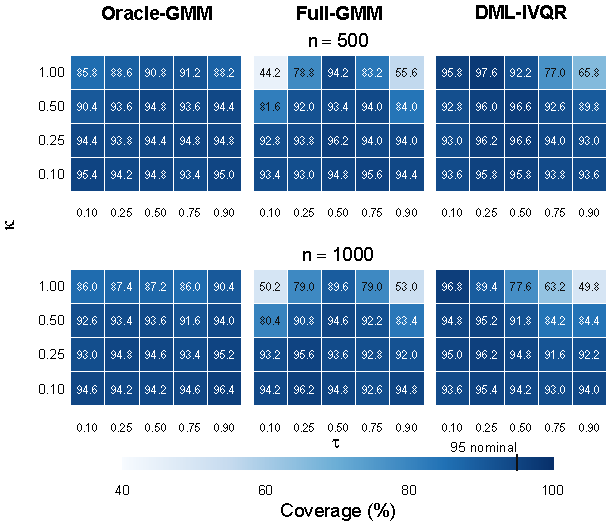
\includegraphics[width=0.72\textwidth]{figures/generated/coverage_heatmap.pdf}
  \caption{Empirical coverage across simulation designs.}
  \label{fig:coverage-heatmap}
  \begin{figurenotes}
    Nominal coverage is 95\%; each cell uses 500 complete replications. Coverage is the fraction of tests accepting the true parameter, evaluated directly at that parameter rather than reconstructed from grid membership. Panel columns identify estimators; panel rows show $n=500$ and $n=1000$. Within each panel, columns show quantiles $\tau$ and rows show relevance $\kappa$, declining from 1.00 to 0.10. Annotations and the common colour scale report percentages. Darker shading indicates higher coverage, not necessarily better calibration.
  \end{figurenotes}
\end{figure}


Increasing the sample size can improve point accuracy without improving calibration. At $\kappa=1$, DML coverage falls from $0.976$ to $0.894$ between $n=500$ and $n=1000$ at $\tau=0.25$, from $0.922$ to $0.776$ at $\tau=0.50$, from $0.770$ to $0.632$ at $\tau=0.75$, and from $0.658$ to $0.498$ at $\tau=0.90$. These changes equal $-8.2$, $-14.6$, $-13.8$, and $-16.0$ percentage points. Section~\ref{sec:results-point-accuracy} found lower RMSE at $n=1000$ in all 60 matched comparisons, so lower observed RMSE of the grid minimiser does not imply that the candidate-specific test has size closer to its nominal level.

Coverage tends to move toward $0.95$ as relevance weakens, but not monotonically in every cell. Averaged over estimators, quantiles, and sample sizes, coverage rises from $0.798$ at $\kappa=1$ to $0.912$, $0.941$, and $0.944$ as $\kappa$ falls. Only 15 of the 30 estimator--sample-size--quantile sequences are nondecreasing at every step. For example, DML coverage at $n=1000$ and $\tau=0.10$ is $0.968$, $0.948$, $0.950$, and $0.936$ across declining $\kappa$, while Full-GMM coverage at $n=500$ and $\tau=0.25$ is $0.788$, $0.920$, $0.938$, and $0.930$. These reversals are generally small compared with the strong-relevance distortions. More importantly, movement toward nominal coverage under weak relevance can result from rejecting candidate values less often overall.

Each rate is based on $R=500$ replications. Its Monte Carlo standard error is
\[
\operatorname{MCSE}(\widehat p)
=
\sqrt{\frac{\widehat p(1-\widehat p)}{R}}.
\]
The maximum MCSE is approximately $0.022$ and the MCSE at $0.95$ is approximately $0.010$. Appendix~\ref{app:coverage-forensic-audit} strengthens this cell-by-cell uncertainty check. Across 60,000 valid direct-at-truth evaluations, 53 pointwise two-sided 95\% Wilson intervals lie wholly below $0.95$, one lies wholly above it, and 66 contain it. No truth statistic is missing or nonfinite. The intervals use integer acceptance counts without a continuity correction; they are pointwise Monte Carlo intervals, not simultaneous or multiplicity-adjusted tests. An individual rate's MCSE is not used as the standard error of a difference between correlated simulation results.

The audit rules out missing-value handling, nonfinite truth statistics, and reconstruction from rounded grid confidence sets as explanations for the observed undercoverage. It does not isolate a cause among finite-sample approximation error, features of the preserved implementation, or failure of the idealised regularity conditions for the asymptotic chi-square reference law in this DGP. Strong-relevance undercoverage also shows that weak relevance alone cannot explain the distortions. Coverage records retention of the truth; it does not record how readily false candidates are excluded. The next two sections therefore examine power and accepted-set informativeness before interpreting near-nominal coverage under weak relevance.

\subsection{Power Against False Candidate Values}
\label{sec:results-power}

Figure~\ref{fig:power-median-combined} reports rejection probabilities at $\tau=0.50$ for candidate values $a_{\Delta}(\tau)=\alpha_0(\tau)+\Delta$. At $\Delta=0$, the candidate is true and rejection probability is empirical size; at each of the six nonzero deviations, it is empirical power against that specified false candidate. The data-generating parameter remains fixed throughout. The plotted probabilities use the same nominal 5\% chi-square cutoff and are not adjusted for differences in empirical size.

\begin{figure}[!htbp]
  \centering
  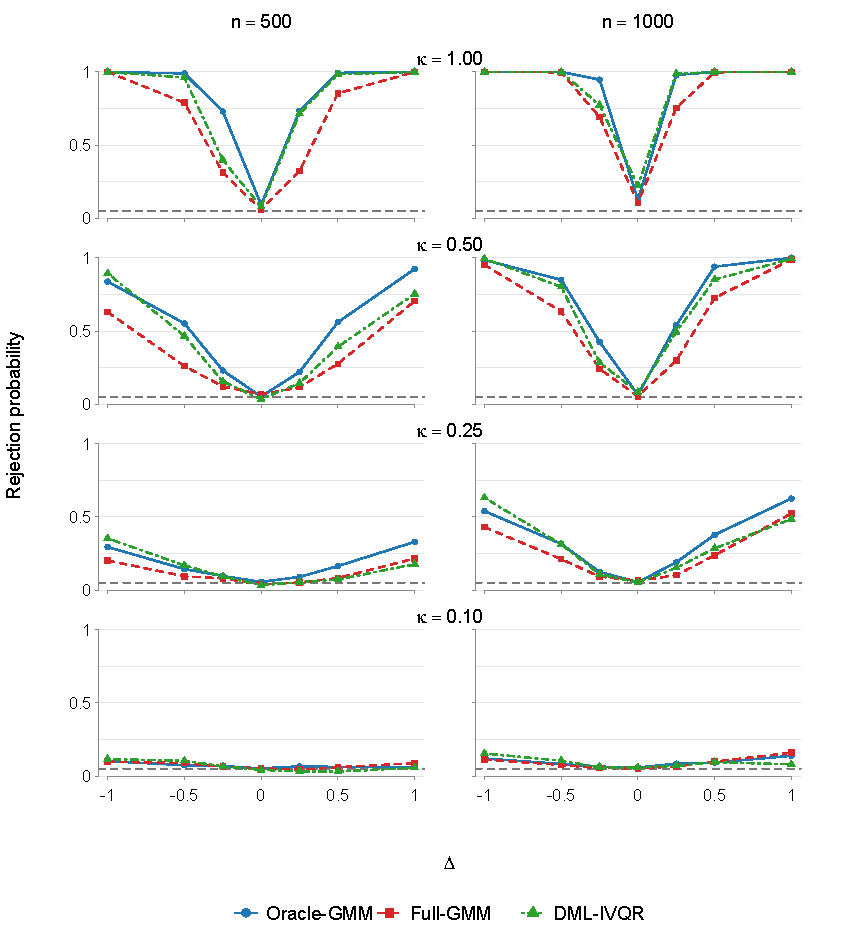
\includegraphics[width=\linewidth]{figures/generated/power_median_combined.pdf}
  \caption{Empirical power at the median.}
  \label{fig:power-median-combined}
  \begin{figurenotes}
    The median benchmark is $\tau=0.50$. Columns show $n=500$ and $n=1000$; rows show $\kappa=1.00,0.50,0.25,0.10$. The horizontal axis is $\Delta=a-\alpha_0(0.50)$, the saved deviation of the tested candidate from truth. Each point uses 500 complete replications and the same nominal 5\% chi-square cutoff; dashed horizontal lines mark 0.05. Rejection at truth is evaluated directly. At $\Delta=0$, rejection probability measures empirical size; at nonzero deviations, it measures power. These rejection probabilities are not size-adjusted. Straight segments are visual guides between evaluated points.
  \end{figurenotes}
\end{figure}


At $n=1000$ and $\Delta=-0.50$, Oracle power falls from $1.000$ through $0.850$ and $0.316$ to $0.082$ as $\kappa$ declines, while DML falls from $1.000$ through $0.802$ and $0.312$ to $0.104$. Full-GMM likewise falls from $0.998$ to $0.076$ between the strongest and weakest settings. For $\Delta=0.50$ at $\kappa=0.25$, power is $0.378$, $0.238$, and $0.286$ for Oracle, Full, and DML, before falling to approximately one tenth for all three at $\kappa=0.10$. The deterioration is therefore already substantial at intermediate relevance, and false effects separated from truth by one half become difficult to exclude in the weakest setting.

Increasing $n$ usually raises power where usable signal remains. At $\kappa=0.50$, Oracle power at $\Delta=-0.50$ rises from $0.552$ to $0.850$, Full from $0.260$ to $0.634$, and DML from $0.466$ to $0.802$ between $n=500$ and $n=1000$. At $\Delta=0.50$, the corresponding changes are $0.560$ to $0.940$, $0.276$ to $0.726$, and $0.392$ to $0.852$. At $\kappa=0.10$, improvements are much smaller and not uniform: Full power at $\Delta=-0.50$ falls from $0.088$ to $0.076$, while DML remains $0.104$; at $\Delta=0.50$, DML rises from $0.030$ to $0.094$. Across all five quantiles and six nonzero deviations, $n=1000$ has higher rejection probability in 305 of 360 matched cells, the same probability in 25, and a lower probability in 30.

The null points clarify why raw power cannot be used as an efficiency ranking. At $n=1000$ and $\kappa=1$, median empirical size is $0.128$ for Oracle, $0.104$ for Full, and $0.224$ for DML, compared with $0.092$, $0.058$, and $0.078$ at $n=500$. DML's strong-relevance rejection of false candidates therefore coexists with the size distortion documented in Section~\ref{sec:results-coverage}. At $n=1000$ and $\kappa=0.10$, empirical sizes are $0.058$, $0.052$, and $0.058$, while power at $\Delta=-0.50$ is only $0.082$, $0.076$, and $0.104$. Rejection of this false candidate is then close to rejection at truth, indicating little discrimination despite approximately nominal size.

The median pattern broadly generalises, but it is not universally monotone. Across all quantiles, sample sizes, estimators, and nonzero deviations, power is nonincreasing as $\kappa$ falls in 162 of 180 sequences. The 18 exceptions are mostly small reversals when rejection is already close to empirical size. Signed differences also occur: for DML at $\tau=0.50$, $n=500$, and $\kappa=0.25$, power is $0.168$ at $\Delta=-0.50$ but $0.072$ at $\Delta=0.50$. Figure~\ref{fig:power-median-combined} displays only $\tau=0.50$, so these full-result counts support generalisation without implying that every quantile follows the plotted paths. The design does not isolate the source of signed asymmetry, and asymmetry in power is not by itself evidence of point-estimation bias.

\FloatBarrier

\subsection{Confidence-Set Informativeness}
\label{sec:results-informativeness}

Figure~\ref{fig:accepted-measure-main} reports the median grid-based accepted-set measure within $A_0=[-1,3]$. The measure increases strictly at every step as $\kappa$ falls in all 30 estimator--sample-size--quantile sequences. At $n=1000$ and $\tau=0.50$, Oracle, Full, and DML medians rise from $0.200$, $0.400$, and $0.300$ at $\kappa=1$ to $3.900$, $3.800$, and $3.900$ at $\kappa=0.10$. Thus declining relevance causes progressively more of the maintained domain to survive test inversion, even when coverage moves closer to $0.95$.

\begin{figure}[!htbp]
  \centering
  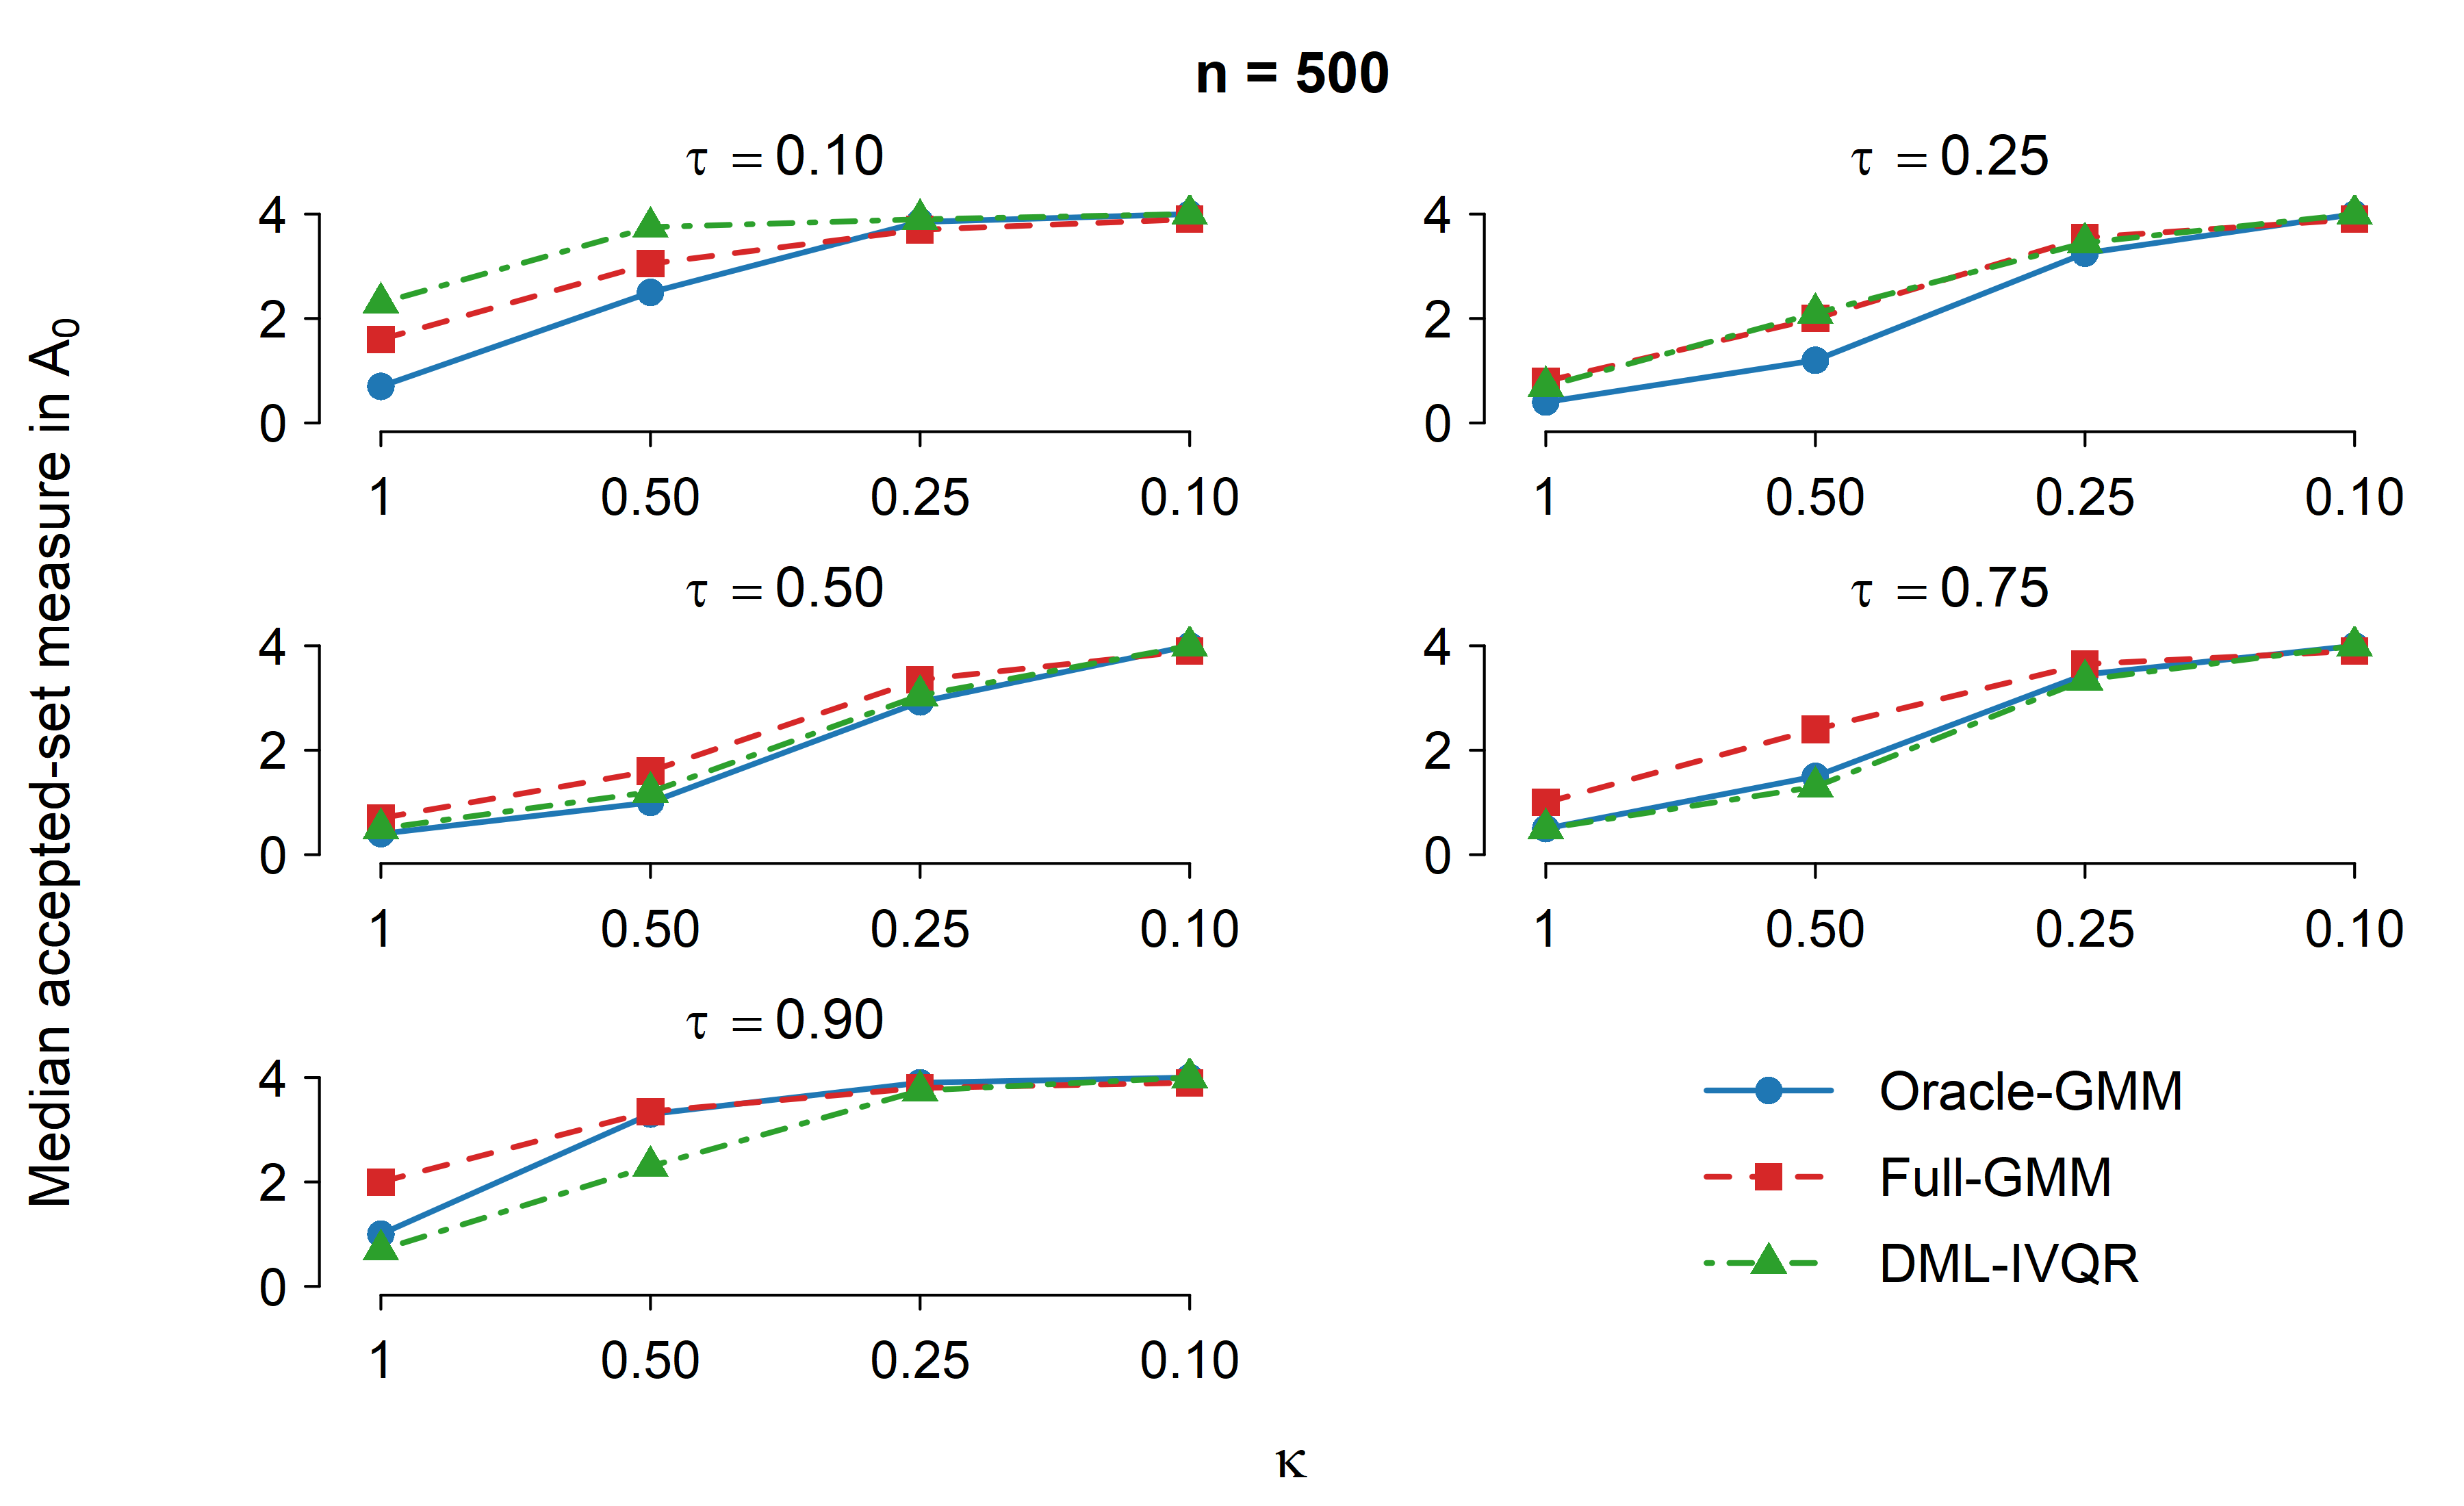
\includegraphics[width=\linewidth]{figures/generated/accepted_measure_n500.png}
  \par\medskip
  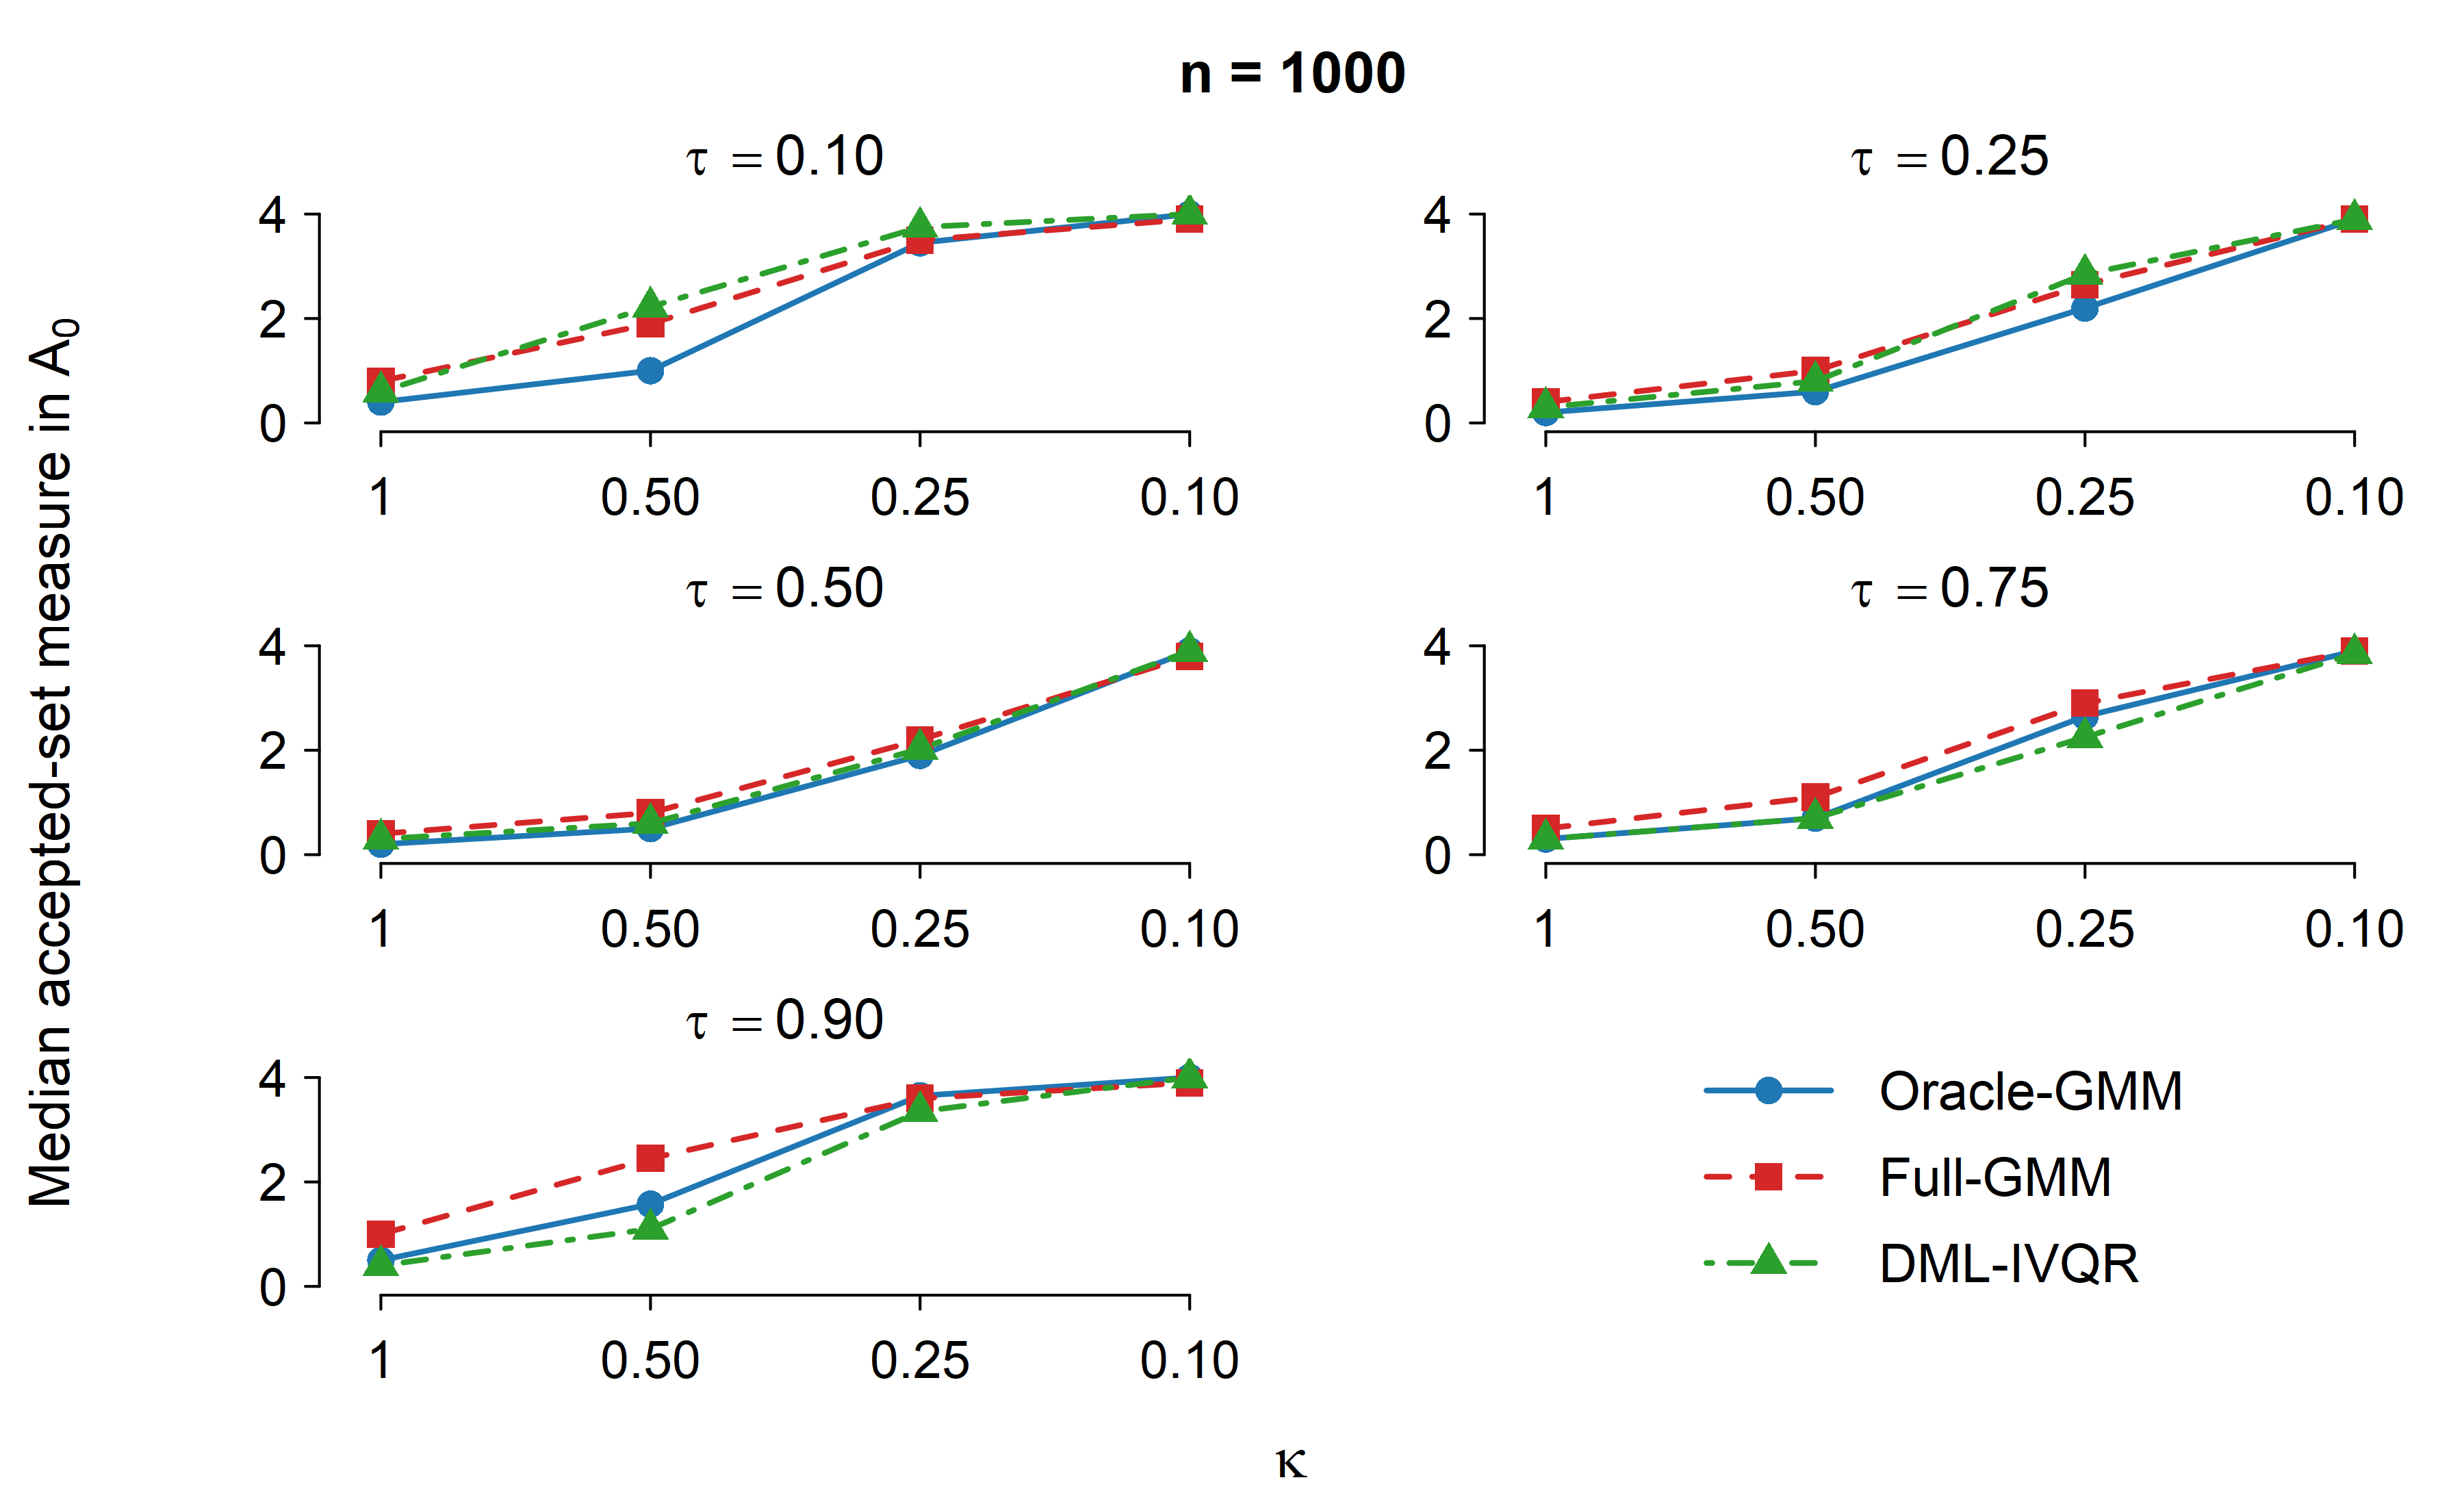
\includegraphics[width=\linewidth]{figures/generated/accepted_measure_n1000.png}
  \caption{Grid-based accepted-set measure within the primary computational domain $A_0=[-1,3]$.}
  \label{fig:accepted-measure-main}

\begin{figurenotes}
Panels show $n=500$ and $n=1000$, using 500 replications per cell. Curves identify Oracle-GMM, Full-GMM, and DML-IVQR; quantile panels show $\tau$. Plotted values are replication medians of the trapezoidal binary-grid-acceptance measure at each $\kappa$. The maximum is four, the width of $A_0$; this is not unrestricted confidence-region length. Lines join evaluated relevance settings as visual guides.
\end{figurenotes}
\end{figure}


Quantile and estimator differences are visible before the weakest setting. At $n=1000$ and $\kappa=0.50$, DML's median measure ranges from $0.600$ at $\tau=0.50$ to $2.225$ at $\tau=0.10$, while Full ranges from $0.800$ to $2.450$ across the five quantiles. Increasing the sample size narrows the median accepted measure in 52 of 60 matched cells and leaves it unchanged in eight; it never widens it. For example, DML at $\tau=0.50$ and $\kappa=0.25$ falls from $3.050$ to $2.025$, whereas at $\kappa=0.10$ it falls only from $4.000$ to $3.900$. More observations improve localisation, but do not overcome the weakest relevance setting at these sample sizes.

The DML sequence at $n=1000$ and $\tau=0.50$ connects the four inferential summaries. At $\kappa=1$, coverage is $0.776$, the median accepted measure is $0.300$, the full-grid acceptance rate is $0.000$, and power at $\Delta=0.50$ is $1.000$. At $\kappa=0.25$, the corresponding values are $0.948$, $2.025$, $0.040$, and $0.286$. At $\kappa=0.10$, coverage remains near nominal at $0.942$, but the median measure is $3.900$, full-grid acceptance is $0.428$, and power at $\Delta=0.50$ is $0.094$. Truth retention, the amount of the grid retained, acceptance of the entire grid, and rejection of a particular false value therefore answer different questions.

The measure cannot exceed four because it integrates grid acceptance only over $A_0=[-1,3]$. Similar values near four do not imply equivalent unrestricted confidence regions: the calculation does not examine candidates outside $A_0$, and distinct acceptance patterns can produce similar totals. Supplementary Figure~\ref{fig:appendix_full_domain_acceptance} records the frequency with which all 41 evaluated points are accepted. That event does not establish acceptance at every intermediate real value or anywhere outside $A_0$. Coverage is also a separate direct evaluation at truth. For DML, fresh pivotal draws mean that direct-truth coverage and stored-profile acceptance need not coincide even when truth is numerically a grid point.

Appendix~\ref{app:numerical-domain-diagnostics} examines wider domains in a separate diagnostic with $n=1000$, 100 replications, all five quantiles and estimators, $\kappa\in\{1,0.25,0.10\}$, and step $0.1$ on $A_0=[-1,3]$, $A_1=[-3,5]$, and $A_2=[-5,7]$. At $\tau=0.50$ and $\kappa=1$, median DML measure remains $0.300$ on all three domains and $A_2$ boundary acceptance is zero. At $\kappa=0.25$, it grows from $1.950$ to $2.500$ and $3.025$, with $A_2$ boundary acceptance $0.500$. At $\kappa=0.10$, it grows from $3.900$ to $7.500$ and $10.325$, and the $A_2$ boundary is accepted in $0.960$ of usable profiles. Oracle and Full display the same broad weak-relevance pattern, with $A_2$ median measures $11.300$ and $11.450$ and boundary rates $0.830$ and $0.850$ in the corresponding cell.

These domain-expansion values come from a diagnostic run with 100 replications, not the main 500-replication experiment. They show near-stability within the investigated domains under strong relevance and continued failure to localise at intermediate and weak relevance. The diagnostic ends at $A_2$ and does not search the real line. Failure to localise over these domains is evidence of limited numerical informativeness, not proof of global unboundedness or non-identification.

\FloatBarrier

\section{Discussion}

\label{sec:results-overall-interpretation}

Taken together, the results show that weakening instrument relevance changes each dimension of finite-sample performance, but not in the same way. Point accuracy deteriorates systematically, accepted sets expand, and power against false candidate values generally declines, subject to the documented small reversals. Coverage is less systematic and can move toward its nominal level precisely when the procedure rejects few candidates. Near-nominal coverage can therefore coexist with low power and acceptance of most or all of the numerical domain. Accuracy, calibration, power, and informativeness measure different features of the procedure, and no one of them is sufficient to assess inference.

The estimator comparison reinforces this interpretation. Oracle-GMM knows the designated relevant controls, yet its point accuracy, power, and accepted-set localisation still deteriorate as relevance declines. High-dimensional nuisance estimation therefore cannot be the sole explanation for the common relevance pattern. DML-IVQR usually has lower RMSE than Full-GMM, but the documented exceptions and the separate coverage and power results rule out uniform superiority. Oracle is likewise an infeasible benchmark rather than a guaranteed finite-sample winner. Because the implementations differ in nuisance dimension, regularisation, and residualisation details, these are comparisons among complete estimator implementations; they do not isolate the causal effect of regularisation.

Sample size and quantile comparisons require similar qualifications. Increasing $n$ from 500 to 1000 lowers RMSE in all 60 matched comparisons and typically narrows accepted sets and raises power where usable signal remains. It does not improve every inferential dimension: several strong-relevance DML coverage rates deteriorate substantially, and power has documented exceptions. Across quantiles, the lower-tail biases are uniformly negative and the upper-tail biases uniformly positive under the convention $\mathrm{Bias}=\alpha_0-\widehat\alpha$. At fixed estimator, $n$, and $\kappa$, both MAE and RMSE are lower at the median than at either tail throughout the final results, whereas coverage has no corresponding universal centre-versus-tail ordering. Results at two sample sizes establish finite-sample contrasts, not an asymptotic rate or limit.

Neyman orthogonality is designed to reduce first-order sensitivity to small nuisance-estimation errors \parencite{chernozhukov_et_al_2018}, while candidate-specific test inversion is designed to avoid relying on a precisely estimated structural coefficient under weak identification \parencite{chernozhukov_hansen_2008}. Neither property creates identifying variation. Subject to its assumptions and regularity conditions, weak-identification-robust construction concerns validity of testing a candidate; it does not promise a narrow confidence region or high power when many false candidates are observationally difficult to distinguish. The DML-IVQR framework of \textcite{chen_huang_tien_2021} combines high-dimensional nuisance estimation with this style of candidate-specific inference, but the present simulations evaluate the preserved executable procedure. They do not validate the ideal asymptotic theory.

The population density weight at the true parameter encounters the non-finite regularity problem derived in Section~\ref{sec:framework}. The executable estimators instead use the fitted-normal density proxy and implementation-specific residualisation rules in Section~\ref{sec:implementation}; Appendix~\ref{app:reproducibility} further records that the preserved \texttt{dnorm} call supplies the residual variance in the argument position interpreted by R as a standard deviation. DML uses the same sample for nuisances and scores rather than cross-fitting, and its pivotal penalty generates fresh draws across evaluations. All three estimators use an asymptotic chi-square reference cutoff, while their empirical sizes differ. These features qualify the relationship between the experiment and the theoretical procedures, but the design does not vary them separately. None can therefore be identified as the cause of a particular distortion, and the results do not establish that changing one feature would remove it.

The numerical and design scope imposes further limits. Point estimates minimize a 41-point profile and hence reflect its resolution, endpoints, and first-tie rule. The accepted-set measure is restricted to $A_0=[-1,3]$ and cannot describe acceptance outside that domain; Appendix~\ref{app:numerical-domain-diagnostics} shows that accepted measure and boundary acceptance can continue to grow on wider investigated domains under weak relevance. Those diagnostics establish limited numerical localisation over the ranges examined, not global unboundedness or non-identification. More broadly, the evidence comes from one DGP family, five quantiles, two sample sizes, four relevance settings, and three preserved estimator implementations. It cannot establish how every alternative DGP, implementation, or larger sample would behave.

The bounded implication is therefore to distinguish what can be assessed in a simulation from what can be established in an empirical application. A procedure can produce a more accurate point estimate while remaining poorly calibrated, attain coverage near the nominal level while excluding few false candidates, or show a finite-domain measure near its ceiling without establishing the shape of an unrestricted confidence region. Simulation evaluations should report accuracy, calibration, power, and informativeness jointly. In empirical applications, researchers should disclose numerical-domain sensitivity and the assumptions underlying inference; nominal confidence levels alone do not establish finite-sample reliability. Within the scope of this experiment, that distinction gives the clearest account of what is lost as instrument relevance weakens.

\section{Conclusion}
This controlled extension of \textcite{chen_huang_tien_2021} documents the loss of estimation accuracy and inferential informativeness as excluded-instrument relevance weakens in a high-dimensional IVQR design. Independent compensating noise keeps the marginal treatment distribution and the relationship generating endogeneity fixed. The deterioration affects Oracle-GMM as well as Full-GMM and DML-IVQR, so high-dimensional nuisance estimation cannot be its sole explanation.

Regularized nuisance estimation often improves point accuracy relative to Full-GMM, with exceptions. Coverage, however, is distinct from accuracy and informativeness: near-nominal truth retention can coexist with acceptance of most of the computational domain and little power against false effects. Strong-relevance undercoverage further prevents reading the nominal confidence level as a finite-sample guarantee. Orthogonalization and regularization can mitigate high-dimensional estimation difficulties, but cannot replace identifying information lost when instrument relevance deteriorates.

The findings concern one DGP family, two sample sizes, five quantiles, and three preserved implementations. Density-weight regularity, residualization differences, same-sample estimation, penalty randomness, asymptotic critical values, and finite domains qualify the link to theoretical DML-IVQR. Future controlled comparisons could vary these features individually, examine a DGP satisfying the density conditions, and add sample sizes with systematic domain checks. Such experiments would assess mechanisms without presuming that a particular change restores calibration; no finite-grid diagnostic alone can establish global boundedness.

\FloatBarrier
\printbibliography[title={References}]
\clearpage
\appendix
\section*{Online supplementary material}
\noindent Appendices A--D provide numerical-domain diagnostics, the controlled-design derivation, the coverage audit, and implementation notes. They are included here to keep all cross-references resolvable in a single review PDF.
\renewcommand{\theequation}{\thesection.\arabic{equation}}
\renewcommand{\thetable}{\thesection.\arabic{table}}
\renewcommand{\thefigure}{\thesection.\arabic{figure}}
\renewcommand{\theHequation}{\thesection.\arabic{equation}}
\renewcommand{\theHtable}{\thesection.\arabic{table}}
\renewcommand{\theHfigure}{\thesection.\arabic{figure}}
\section{Numerical-Domain Diagnostics}
\setcounter{equation}{0}\setcounter{table}{0}\setcounter{figure}{0}
\label{app:numerical-domain-diagnostics}

\label{app:domain-choice}

The primary computational domain is \(A_0=[-1,3]\), evaluated on 41 equally spaced candidate values with step size \(h=0.1\). 
Using the same domain for all sample sizes, quantiles, instrument-relevance settings, and estimators makes the accepted-set measures directly comparable across the simulation design.

The interval also contains the true structural quantile effects for all five investigated quantiles. Under the data-generating process,
\[
\alpha_0(\tau)=1+\Phi^{-1}(\tau),
\]
so the true effects are approximately \(-0.282\), \(0.326\), \(1.000\), \(1.674\), and \(2.282\) for \(\tau=0.10,0.25,0.50,0.75,\) and \(0.90\), respectively. All five structural truths lie strictly inside \(A_0\); using their unrounded values, the minimum distance to either endpoint is approximately \(0.718\). The interval should therefore be understood as a common numerical search domain, not as an assumed theoretical parameter space.

A finite search domain can nevertheless become restrictive when instruments are weak and many candidate values are accepted. For this reason, a separate sensitivity diagnostic expands the search range from \(A_0=[-1,3]\) to \(A_1=[-3,5]\) and then to \(A_2=[-5,7]\). Under strong instrument relevance, expanding the domain adds little accepted measure, indicating that the observed accepted components are well localized within the investigated ranges. At intermediate relevance, the wider domains contain additional accepted values in some profiles. Under the weakest relevance setting, the accepted measure continues to increase as the domain is expanded and does not stabilize within \(A_2\).

These results clarify the interpretation of the main accepted-set measure. A value close to four in \(A_0\) means that almost the entire four-unit primary domain is accepted; it does not mean that the unrestricted confidence region has length four. Similarly, continued acceptance in the wider domains indicates poor numerical localization over the ranges examined, but it does not by itself establish that the theoretical confidence region is globally unbounded or that identification completely fails.

Table~\ref{tab:appendix-grid-measures} retains the key frozen domain-measure comparisons; Figure~\ref{fig:grid-domain} summarizes the expansion pattern.


The main diagnostic contains one singular-design error: replication 35, $\tau=0.90$, $\kappa=0.10$, DML-IVQR, candidate $a=-2.1$ in Stage 1. Stage 2 adds no new evaluation errors. Incomplete profiles receive missing aggregate measures; the affected expanded-domain cell therefore uses 99 usable replications, while other displayed cells use 100. Tables~\ref{tab:appendix-grid-added}--\ref{tab:appendix-grid-status} retain incremental measures, boundary frequencies, profile counts, and localization diagnostics. In these tables, Med. and Mean denote replication medians and means; $R$ is the intended replication count, Succ. counts complete profiles, Fail counts incomplete profiles, and Stage 1/2 counts newly recorded evaluation errors. Boundary frequencies refer to acceptance of either endpoint; full-grid frequencies require acceptance at every evaluated point. A nonaccepted boundary does not rule out disconnected accepted components farther outside the examined interval.
\begingroup
\begin{booktabs}[
  caption = {Grid-domain diagnostic: accepted-set measures},
  label = {tab:appendix-grid-measures},
  long,
  remark{Note} = {Domains are $A_0=[-1,3]$, $A_1=[-3,5]$, and $A_2=[-5,7]$. Diagnostics concern only these investigated numerical domains and do not establish global boundedness, unboundedness, or disconnected components.}
]{
  colspec = {Q[c] Q[c] Q[c] X[l] *{6}{Q[r]}},
  columns = {colsep = 1pt},
  row{1} = {font = \bfseries},
  rowhead = 1
}
$n$ & $\tau$ & $\kappa$ & Estimator & Med. $A_0$ & Med. $A_1$ & Med. $A_2$ & Mean $A_0$ & Mean $A_1$ & Mean $A_2$ \\
1000 & 0.10 & 1.00 & Oracle-GMM & 0.400 & 0.400 & 0.400 & 0.386 & 0.386 & 0.386 \\
1000 & 0.10 & 1.00 & Full-GMM & 0.800 & 0.800 & 0.800 & 0.757 & 0.757 & 0.757 \\
1000 & 0.10 & 1.00 & DML-IVQR & 0.600 & 0.600 & 0.600 & 0.705 & 0.705 & 0.705 \\
1000 & 0.10 & 0.25 & Oracle-GMM & 3.400 & 5.325 & 7.250 & 3.019 & 4.994 & 6.838 \\
1000 & 0.10 & 0.25 & Full-GMM & 3.375 & 5.950 & 8.200 & 3.304 & 5.774 & 8.037 \\
1000 & 0.10 & 0.25 & DML-IVQR & 3.750 & 5.950 & 7.950 & 3.607 & 6.040 & 8.245 \\
1000 & 0.10 & 0.10 & Oracle-GMM & 4.000 & 7.900 & 11.900 & 3.745 & 7.381 & 11.002 \\
1000 & 0.10 & 0.10 & Full-GMM & 3.900 & 7.800 & 11.600 & 3.785 & 7.394 & 10.975 \\
1000 & 0.10 & 0.10 & DML-IVQR & 4.000 & 7.575 & 10.775 & 3.845 & 7.219 & 10.339 \\
1000 & 0.25 & 1.00 & Oracle-GMM & 0.300 & 0.300 & 0.300 & 0.259 & 0.259 & 0.259 \\
1000 & 0.25 & 1.00 & Full-GMM & 0.400 & 0.400 & 0.400 & 0.429 & 0.429 & 0.429 \\
1000 & 0.25 & 1.00 & DML-IVQR & 0.300 & 0.300 & 0.300 & 0.346 & 0.346 & 0.346 \\
1000 & 0.25 & 0.25 & Oracle-GMM & 2.175 & 2.800 & 2.850 & 2.224 & 3.158 & 3.964 \\
1000 & 0.25 & 0.25 & Full-GMM & 2.450 & 3.500 & 4.075 & 2.517 & 3.768 & 4.745 \\
1000 & 0.25 & 0.25 & DML-IVQR & 2.750 & 4.650 & 6.225 & 2.630 & 4.130 & 5.712 \\
1000 & 0.25 & 0.10 & Oracle-GMM & 3.900 & 7.700 & 11.500 & 3.492 & 6.699 & 9.872 \\
1000 & 0.25 & 0.10 & Full-GMM & 3.825 & 7.600 & 11.100 & 3.595 & 6.891 & 10.083 \\
1000 & 0.25 & 0.10 & DML-IVQR & 4.000 & 7.700 & 11.125 & 3.651 & 6.926 & 9.984 \\
1000 & 0.50 & 1.00 & Oracle-GMM & 0.200 & 0.200 & 0.200 & 0.235 & 0.235 & 0.235 \\
1000 & 0.50 & 1.00 & Full-GMM & 0.400 & 0.400 & 0.400 & 0.373 & 0.373 & 0.373 \\
1000 & 0.50 & 1.00 & DML-IVQR & 0.300 & 0.300 & 0.300 & 0.259 & 0.259 & 0.259 \\
1000 & 0.50 & 0.25 & Oracle-GMM & 1.875 & 2.200 & 2.200 & 1.960 & 2.682 & 3.229 \\
1000 & 0.50 & 0.25 & Full-GMM & 2.250 & 2.400 & 2.550 & 2.368 & 3.171 & 3.802 \\
1000 & 0.50 & 0.25 & DML-IVQR & 1.950 & 2.500 & 3.025 & 2.124 & 3.020 & 3.942 \\
1000 & 0.50 & 0.10 & Oracle-GMM & 3.825 & 7.600 & 11.300 & 3.521 & 6.640 & 9.687 \\
1000 & 0.50 & 0.10 & Full-GMM & 3.900 & 7.625 & 11.450 & 3.536 & 6.718 & 9.817 \\
1000 & 0.50 & 0.10 & DML-IVQR & 3.900 & 7.500 & 10.325 & 3.538 & 6.671 & 9.585 \\
1000 & 0.75 & 1.00 & Oracle-GMM & 0.300 & 0.300 & 0.300 & 0.290 & 0.290 & 0.290 \\
1000 & 0.75 & 1.00 & Full-GMM & 0.500 & 0.500 & 0.500 & 0.512 & 0.512 & 0.512 \\
1000 & 0.75 & 1.00 & DML-IVQR & 0.300 & 0.300 & 0.300 & 0.279 & 0.279 & 0.279 \\
1000 & 0.75 & 0.25 & Oracle-GMM & 2.825 & 4.200 & 4.850 & 2.628 & 3.945 & 4.990 \\
1000 & 0.75 & 0.25 & Full-GMM & 2.950 & 4.450 & 5.150 & 2.827 & 4.267 & 5.478 \\
1000 & 0.75 & 0.25 & DML-IVQR & 2.325 & 3.300 & 3.900 & 2.402 & 3.595 & 4.788 \\
1000 & 0.75 & 0.10 & Oracle-GMM & 3.975 & 7.750 & 11.700 & 3.670 & 6.999 & 10.357 \\
1000 & 0.75 & 0.10 & Full-GMM & 3.900 & 7.750 & 11.500 & 3.661 & 7.023 & 10.267 \\
1000 & 0.75 & 0.10 & DML-IVQR & 3.900 & 7.350 & 10.375 & 3.554 & 6.691 & 9.736 \\
1000 & 0.90 & 1.00 & Oracle-GMM & 0.500 & 0.500 & 0.500 & 0.519 & 0.519 & 0.519 \\
1000 & 0.90 & 1.00 & Full-GMM & 1.000 & 1.000 & 1.000 & 1.026 & 1.031 & 1.031 \\
1000 & 0.90 & 1.00 & DML-IVQR & 0.400 & 0.400 & 0.400 & 0.454 & 0.454 & 0.454 \\
1000 & 0.90 & 0.25 & Oracle-GMM & 3.650 & 5.850 & 7.850 & 3.381 & 5.625 & 7.675 \\
1000 & 0.90 & 0.25 & Full-GMM & 3.675 & 6.150 & 8.575 & 3.555 & 6.123 & 8.432 \\
1000 & 0.90 & 0.25 & DML-IVQR & 3.450 & 5.400 & 7.300 & 3.114 & 5.249 & 7.374 \\
1000 & 0.90 & 0.10 & Oracle-GMM & 4.000 & 7.900 & 11.800 & 3.712 & 7.241 & 10.771 \\
1000 & 0.90 & 0.10 & Full-GMM & 3.900 & 7.700 & 11.500 & 3.817 & 7.448 & 11.031 \\
1000 & 0.90 & 0.10 & DML-IVQR & 4.000 & 7.700 & 11.600 & 3.644 & 7.042 & 10.395 \\
\end{booktabs}
\endgroup
\clearpage
\begingroup
\begin{booktabs}[
  caption = {Grid-domain diagnostic: added accepted measure},
  label = {tab:appendix-grid-added},
  long,
  remark{Note} = {Domains are $A_0=[-1,3]$, $A_1=[-3,5]$, and $A_2=[-5,7]$. Diagnostics concern only these investigated numerical domains and do not establish global boundedness, unboundedness, or disconnected components.}
]{
  colspec = {Q[c] Q[c] Q[c] X[l] Q[r] Q[r] Q[r] Q[r]},
  columns = {colsep = 1.5pt},
  row{1} = {font = \bfseries},
  rowhead = 1
}
$n$ & $\tau$ & $\kappa$ & Estimator & Med. $A_0\to A_1$ & Mean $A_0\to A_1$ & Med. $A_1\to A_2$ & Mean $A_1\to A_2$ \\
1000 & 0.10 & 1.00 & Oracle-GMM & 0.000 & 0.000 & 0.000 & 0.000 \\
1000 & 0.10 & 1.00 & Full-GMM & 0.000 & 0.000 & 0.000 & 0.000 \\
1000 & 0.10 & 1.00 & DML-IVQR & 0.000 & 0.000 & 0.000 & 0.000 \\
1000 & 0.10 & 0.25 & Oracle-GMM & 2.000 & 1.974 & 2.000 & 1.844 \\
1000 & 0.10 & 0.25 & Full-GMM & 2.500 & 2.470 & 2.200 & 2.263 \\
1000 & 0.10 & 0.25 & DML-IVQR & 2.150 & 2.433 & 2.000 & 2.205 \\
1000 & 0.10 & 0.10 & Oracle-GMM & 4.000 & 3.636 & 4.000 & 3.621 \\
1000 & 0.10 & 0.10 & Full-GMM & 3.850 & 3.610 & 3.875 & 3.580 \\
1000 & 0.10 & 0.10 & DML-IVQR & 3.700 & 3.374 & 3.450 & 3.120 \\
1000 & 0.25 & 1.00 & Oracle-GMM & 0.000 & 0.000 & 0.000 & 0.000 \\
1000 & 0.25 & 1.00 & Full-GMM & 0.000 & 0.000 & 0.000 & 0.000 \\
1000 & 0.25 & 1.00 & DML-IVQR & 0.000 & 0.000 & 0.000 & 0.000 \\
1000 & 0.25 & 0.25 & Oracle-GMM & 0.275 & 0.933 & 0.000 & 0.806 \\
1000 & 0.25 & 0.25 & Full-GMM & 1.025 & 1.251 & 0.600 & 0.978 \\
1000 & 0.25 & 0.25 & DML-IVQR & 1.750 & 1.500 & 2.000 & 1.582 \\
1000 & 0.25 & 0.10 & Oracle-GMM & 3.900 & 3.207 & 3.900 & 3.174 \\
1000 & 0.25 & 0.10 & Full-GMM & 3.800 & 3.296 & 3.800 & 3.192 \\
1000 & 0.25 & 0.10 & DML-IVQR & 3.950 & 3.275 & 3.625 & 3.058 \\
1000 & 0.50 & 1.00 & Oracle-GMM & 0.000 & 0.000 & 0.000 & 0.000 \\
1000 & 0.50 & 1.00 & Full-GMM & 0.000 & 0.000 & 0.000 & 0.000 \\
1000 & 0.50 & 1.00 & DML-IVQR & 0.000 & 0.000 & 0.000 & 0.000 \\
1000 & 0.50 & 0.25 & Oracle-GMM & 0.000 & 0.722 & 0.000 & 0.547 \\
1000 & 0.50 & 0.25 & Full-GMM & 0.100 & 0.803 & 0.000 & 0.630 \\
1000 & 0.50 & 0.25 & DML-IVQR & 0.250 & 0.895 & 0.400 & 0.921 \\
1000 & 0.50 & 0.10 & Oracle-GMM & 3.900 & 3.119 & 4.000 & 3.047 \\
1000 & 0.50 & 0.10 & Full-GMM & 3.900 & 3.182 & 3.900 & 3.099 \\
1000 & 0.50 & 0.10 & DML-IVQR & 3.850 & 3.134 & 2.850 & 2.914 \\
1000 & 0.75 & 1.00 & Oracle-GMM & 0.000 & 0.000 & 0.000 & 0.000 \\
1000 & 0.75 & 1.00 & Full-GMM & 0.000 & 0.000 & 0.000 & 0.000 \\
1000 & 0.75 & 1.00 & DML-IVQR & 0.000 & 0.000 & 0.000 & 0.000 \\
1000 & 0.75 & 0.25 & Oracle-GMM & 1.325 & 1.317 & 0.400 & 1.045 \\
1000 & 0.75 & 0.25 & Full-GMM & 1.375 & 1.440 & 0.900 & 1.211 \\
1000 & 0.75 & 0.25 & DML-IVQR & 0.525 & 1.193 & 1.200 & 1.192 \\
1000 & 0.75 & 0.10 & Oracle-GMM & 4.000 & 3.329 & 4.000 & 3.358 \\
1000 & 0.75 & 0.10 & Full-GMM & 3.900 & 3.362 & 3.800 & 3.244 \\
1000 & 0.75 & 0.10 & DML-IVQR & 3.575 & 3.136 & 3.600 & 3.045 \\
1000 & 0.90 & 1.00 & Oracle-GMM & 0.000 & 0.000 & 0.000 & 0.000 \\
1000 & 0.90 & 1.00 & Full-GMM & 0.000 & 0.005 & 0.000 & 0.000 \\
1000 & 0.90 & 1.00 & DML-IVQR & 0.000 & 0.000 & 0.000 & 0.000 \\
1000 & 0.90 & 0.25 & Oracle-GMM & 2.050 & 2.244 & 2.000 & 2.050 \\
1000 & 0.90 & 0.25 & Full-GMM & 2.600 & 2.568 & 2.200 & 2.309 \\
1000 & 0.90 & 0.25 & DML-IVQR & 2.000 & 2.135 & 2.000 & 2.125 \\
1000 & 0.90 & 0.10 & Oracle-GMM & 4.000 & 3.529 & 4.000 & 3.530 \\
1000 & 0.90 & 0.10 & Full-GMM & 3.800 & 3.631 & 3.825 & 3.583 \\
1000 & 0.90 & 0.10 & DML-IVQR & 4.000 & 3.399 & 4.000 & 3.353 \\
\end{booktabs}
\endgroup
\clearpage
\begingroup
\begin{booktabs}[
  caption = {Grid-domain diagnostic: boundary and full-grid acceptance},
  label = {tab:appendix-grid-boundary},
  long,
  remark{Note} = {Domains are $A_0=[-1,3]$, $A_1=[-3,5]$, and $A_2=[-5,7]$. Diagnostics concern only these investigated numerical domains and do not establish global boundedness, unboundedness, or disconnected components.}
]{
  colspec = {Q[c] Q[c] Q[c] X[l] *{6}{Q[r]}},
  columns = {colsep = 1pt},
  row{1} = {font = \bfseries},
  rowhead = 1
}
$n$ & $\tau$ & $\kappa$ & Estimator & Boundary $A_0$ & Boundary $A_1$ & Boundary $A_2$ & All $A_0$ & All $A_1$ & All $A_2$ \\
1000 & 0.10 & 1.00 & Oracle-GMM & 0.000 & 0.000 & 0.000 & 0.000 & 0.000 & 0.000 \\
1000 & 0.10 & 1.00 & Full-GMM & 0.000 & 0.000 & 0.000 & 0.000 & 0.000 & 0.000 \\
1000 & 0.10 & 1.00 & DML-IVQR & 0.000 & 0.000 & 0.000 & 0.000 & 0.000 & 0.000 \\
1000 & 0.10 & 0.25 & Oracle-GMM & 0.880 & 0.770 & 0.740 & 0.150 & 0.070 & 0.050 \\
1000 & 0.10 & 0.25 & Full-GMM & 0.920 & 0.840 & 0.750 & 0.090 & 0.030 & 0.020 \\
1000 & 0.10 & 0.25 & DML-IVQR & 0.950 & 0.980 & 0.980 & 0.240 & 0.060 & 0.050 \\
1000 & 0.10 & 0.10 & Oracle-GMM & 1.000 & 1.000 & 1.000 & 0.580 & 0.430 & 0.390 \\
1000 & 0.10 & 0.10 & Full-GMM & 0.990 & 0.980 & 0.990 & 0.430 & 0.210 & 0.150 \\
1000 & 0.10 & 0.10 & DML-IVQR & 1.000 & 0.990 & 0.990 & 0.560 & 0.260 & 0.200 \\
1000 & 0.25 & 1.00 & Oracle-GMM & 0.000 & 0.000 & 0.000 & 0.000 & 0.000 & 0.000 \\
1000 & 0.25 & 1.00 & Full-GMM & 0.000 & 0.000 & 0.000 & 0.000 & 0.000 & 0.000 \\
1000 & 0.25 & 1.00 & DML-IVQR & 0.000 & 0.000 & 0.000 & 0.000 & 0.000 & 0.000 \\
1000 & 0.25 & 0.25 & Oracle-GMM & 0.400 & 0.360 & 0.270 & 0.070 & 0.050 & 0.030 \\
1000 & 0.25 & 0.25 & Full-GMM & 0.560 & 0.390 & 0.390 & 0.060 & 0.030 & 0.010 \\
1000 & 0.25 & 0.25 & DML-IVQR & 0.610 & 0.740 & 0.740 & 0.090 & 0.050 & 0.020 \\
1000 & 0.25 & 0.10 & Oracle-GMM & 0.940 & 0.930 & 0.940 & 0.470 & 0.380 & 0.320 \\
1000 & 0.25 & 0.10 & Full-GMM & 0.960 & 0.930 & 0.900 & 0.320 & 0.250 & 0.210 \\
1000 & 0.25 & 0.10 & DML-IVQR & 0.980 & 0.990 & 0.990 & 0.550 & 0.400 & 0.290 \\
1000 & 0.50 & 1.00 & Oracle-GMM & 0.000 & 0.000 & 0.000 & 0.000 & 0.000 & 0.000 \\
1000 & 0.50 & 1.00 & Full-GMM & 0.000 & 0.000 & 0.000 & 0.000 & 0.000 & 0.000 \\
1000 & 0.50 & 1.00 & DML-IVQR & 0.000 & 0.000 & 0.000 & 0.000 & 0.000 & 0.000 \\
1000 & 0.50 & 0.25 & Oracle-GMM & 0.390 & 0.200 & 0.150 & 0.050 & 0.040 & 0.020 \\
1000 & 0.50 & 0.25 & Full-GMM & 0.400 & 0.240 & 0.260 & 0.050 & 0.020 & 0.020 \\
1000 & 0.50 & 0.25 & DML-IVQR & 0.440 & 0.340 & 0.500 & 0.060 & 0.020 & 0.020 \\
1000 & 0.50 & 0.10 & Oracle-GMM & 0.910 & 0.890 & 0.830 & 0.420 & 0.350 & 0.320 \\
1000 & 0.50 & 0.10 & Full-GMM & 0.940 & 0.890 & 0.850 & 0.450 & 0.320 & 0.280 \\
1000 & 0.50 & 0.10 & DML-IVQR & 0.900 & 0.930 & 0.960 & 0.450 & 0.360 & 0.300 \\
1000 & 0.75 & 1.00 & Oracle-GMM & 0.000 & 0.000 & 0.000 & 0.000 & 0.000 & 0.000 \\
1000 & 0.75 & 1.00 & Full-GMM & 0.000 & 0.000 & 0.000 & 0.000 & 0.000 & 0.000 \\
1000 & 0.75 & 1.00 & DML-IVQR & 0.000 & 0.000 & 0.000 & 0.000 & 0.000 & 0.000 \\
1000 & 0.75 & 0.25 & Oracle-GMM & 0.620 & 0.470 & 0.370 & 0.070 & 0.050 & 0.040 \\
1000 & 0.75 & 0.25 & Full-GMM & 0.650 & 0.550 & 0.530 & 0.080 & 0.010 & 0.000 \\
1000 & 0.75 & 0.25 & DML-IVQR & 0.550 & 0.450 & 0.550 & 0.090 & 0.060 & 0.030 \\
1000 & 0.75 & 0.10 & Oracle-GMM & 0.940 & 0.960 & 0.930 & 0.500 & 0.400 & 0.380 \\
1000 & 0.75 & 0.10 & Full-GMM & 0.980 & 0.920 & 0.920 & 0.420 & 0.270 & 0.220 \\
1000 & 0.75 & 0.10 & DML-IVQR & 0.950 & 0.970 & 0.980 & 0.470 & 0.360 & 0.310 \\
1000 & 0.90 & 1.00 & Oracle-GMM & 0.000 & 0.000 & 0.000 & 0.000 & 0.000 & 0.000 \\
1000 & 0.90 & 1.00 & Full-GMM & 0.000 & 0.000 & 0.000 & 0.000 & 0.000 & 0.000 \\
1000 & 0.90 & 1.00 & DML-IVQR & 0.000 & 0.000 & 0.000 & 0.000 & 0.000 & 0.000 \\
1000 & 0.90 & 0.25 & Oracle-GMM & 0.850 & 0.760 & 0.760 & 0.250 & 0.090 & 0.060 \\
1000 & 0.90 & 0.25 & Full-GMM & 0.960 & 0.800 & 0.820 & 0.110 & 0.060 & 0.030 \\
1000 & 0.90 & 0.25 & DML-IVQR & 0.820 & 0.770 & 0.790 & 0.210 & 0.100 & 0.060 \\
1000 & 0.90 & 0.10 & Oracle-GMM & 0.980 & 1.000 & 1.000 & 0.620 & 0.450 & 0.430 \\
1000 & 0.90 & 0.10 & Full-GMM & 1.000 & 0.990 & 0.990 & 0.380 & 0.110 & 0.060 \\
1000 & 0.90 & 0.10 & DML-IVQR & 0.990 & 0.980 & 0.990 & 0.510 & 0.394 & 0.343 \\
\end{booktabs}
\endgroup
\clearpage
\begingroup
\begin{booktabs}[
  caption = {Grid-domain diagnostic: profiles and numerical errors},
  label = {tab:appendix-grid-profiles},
  long,
  remark{Note} = {Domains are $A_0=[-1,3]$, $A_1=[-3,5]$, and $A_2=[-5,7]$. Diagnostics concern only these investigated numerical domains and do not establish global boundedness, unboundedness, or disconnected components.}
]{
  colspec = {Q[c] Q[c] Q[c] X[l] *{9}{Q[r]}},
  columns = {colsep = .7pt},
  row{1} = {font = \bfseries},
  rowhead = 1
}
$n$ & $\tau$ & $\kappa$ & Estimator & $R$ & \shortstack{Succ.\\$A_0$} & \shortstack{Succ.\\$A_1$} & \shortstack{Succ.\\$A_2$} & \shortstack{Fail\\$A_0$} & \shortstack{Fail\\$A_1$} & \shortstack{Fail\\$A_2$} & \shortstack{Stage\\1} & \shortstack{Stage\\2} \\
1000 & 0.10 & 1.00 & Oracle-GMM & 100 & 100 & 100 & 100 & 0 & 0 & 0 & 0 & 0 \\
1000 & 0.10 & 1.00 & Full-GMM & 100 & 100 & 100 & 100 & 0 & 0 & 0 & 0 & 0 \\
1000 & 0.10 & 1.00 & DML-IVQR & 100 & 100 & 100 & 100 & 0 & 0 & 0 & 0 & 0 \\
1000 & 0.10 & 0.25 & Oracle-GMM & 100 & 100 & 100 & 100 & 0 & 0 & 0 & 0 & 0 \\
1000 & 0.10 & 0.25 & Full-GMM & 100 & 100 & 100 & 100 & 0 & 0 & 0 & 0 & 0 \\
1000 & 0.10 & 0.25 & DML-IVQR & 100 & 100 & 100 & 100 & 0 & 0 & 0 & 0 & 0 \\
1000 & 0.10 & 0.10 & Oracle-GMM & 100 & 100 & 100 & 100 & 0 & 0 & 0 & 0 & 0 \\
1000 & 0.10 & 0.10 & Full-GMM & 100 & 100 & 100 & 100 & 0 & 0 & 0 & 0 & 0 \\
1000 & 0.10 & 0.10 & DML-IVQR & 100 & 100 & 100 & 100 & 0 & 0 & 0 & 0 & 0 \\
1000 & 0.25 & 1.00 & Oracle-GMM & 100 & 100 & 100 & 100 & 0 & 0 & 0 & 0 & 0 \\
1000 & 0.25 & 1.00 & Full-GMM & 100 & 100 & 100 & 100 & 0 & 0 & 0 & 0 & 0 \\
1000 & 0.25 & 1.00 & DML-IVQR & 100 & 100 & 100 & 100 & 0 & 0 & 0 & 0 & 0 \\
1000 & 0.25 & 0.25 & Oracle-GMM & 100 & 100 & 100 & 100 & 0 & 0 & 0 & 0 & 0 \\
1000 & 0.25 & 0.25 & Full-GMM & 100 & 100 & 100 & 100 & 0 & 0 & 0 & 0 & 0 \\
1000 & 0.25 & 0.25 & DML-IVQR & 100 & 100 & 100 & 100 & 0 & 0 & 0 & 0 & 0 \\
1000 & 0.25 & 0.10 & Oracle-GMM & 100 & 100 & 100 & 100 & 0 & 0 & 0 & 0 & 0 \\
1000 & 0.25 & 0.10 & Full-GMM & 100 & 100 & 100 & 100 & 0 & 0 & 0 & 0 & 0 \\
1000 & 0.25 & 0.10 & DML-IVQR & 100 & 100 & 100 & 100 & 0 & 0 & 0 & 0 & 0 \\
1000 & 0.50 & 1.00 & Oracle-GMM & 100 & 100 & 100 & 100 & 0 & 0 & 0 & 0 & 0 \\
1000 & 0.50 & 1.00 & Full-GMM & 100 & 100 & 100 & 100 & 0 & 0 & 0 & 0 & 0 \\
1000 & 0.50 & 1.00 & DML-IVQR & 100 & 100 & 100 & 100 & 0 & 0 & 0 & 0 & 0 \\
1000 & 0.50 & 0.25 & Oracle-GMM & 100 & 100 & 100 & 100 & 0 & 0 & 0 & 0 & 0 \\
1000 & 0.50 & 0.25 & Full-GMM & 100 & 100 & 100 & 100 & 0 & 0 & 0 & 0 & 0 \\
1000 & 0.50 & 0.25 & DML-IVQR & 100 & 100 & 100 & 100 & 0 & 0 & 0 & 0 & 0 \\
1000 & 0.50 & 0.10 & Oracle-GMM & 100 & 100 & 100 & 100 & 0 & 0 & 0 & 0 & 0 \\
1000 & 0.50 & 0.10 & Full-GMM & 100 & 100 & 100 & 100 & 0 & 0 & 0 & 0 & 0 \\
1000 & 0.50 & 0.10 & DML-IVQR & 100 & 100 & 100 & 100 & 0 & 0 & 0 & 0 & 0 \\
1000 & 0.75 & 1.00 & Oracle-GMM & 100 & 100 & 100 & 100 & 0 & 0 & 0 & 0 & 0 \\
1000 & 0.75 & 1.00 & Full-GMM & 100 & 100 & 100 & 100 & 0 & 0 & 0 & 0 & 0 \\
1000 & 0.75 & 1.00 & DML-IVQR & 100 & 100 & 100 & 100 & 0 & 0 & 0 & 0 & 0 \\
1000 & 0.75 & 0.25 & Oracle-GMM & 100 & 100 & 100 & 100 & 0 & 0 & 0 & 0 & 0 \\
1000 & 0.75 & 0.25 & Full-GMM & 100 & 100 & 100 & 100 & 0 & 0 & 0 & 0 & 0 \\
1000 & 0.75 & 0.25 & DML-IVQR & 100 & 100 & 100 & 100 & 0 & 0 & 0 & 0 & 0 \\
1000 & 0.75 & 0.10 & Oracle-GMM & 100 & 100 & 100 & 100 & 0 & 0 & 0 & 0 & 0 \\
1000 & 0.75 & 0.10 & Full-GMM & 100 & 100 & 100 & 100 & 0 & 0 & 0 & 0 & 0 \\
1000 & 0.75 & 0.10 & DML-IVQR & 100 & 100 & 100 & 100 & 0 & 0 & 0 & 0 & 0 \\
1000 & 0.90 & 1.00 & Oracle-GMM & 100 & 100 & 100 & 100 & 0 & 0 & 0 & 0 & 0 \\
1000 & 0.90 & 1.00 & Full-GMM & 100 & 100 & 100 & 100 & 0 & 0 & 0 & 0 & 0 \\
1000 & 0.90 & 1.00 & DML-IVQR & 100 & 100 & 100 & 100 & 0 & 0 & 0 & 0 & 0 \\
1000 & 0.90 & 0.25 & Oracle-GMM & 100 & 100 & 100 & 100 & 0 & 0 & 0 & 0 & 0 \\
1000 & 0.90 & 0.25 & Full-GMM & 100 & 100 & 100 & 100 & 0 & 0 & 0 & 0 & 0 \\
1000 & 0.90 & 0.25 & DML-IVQR & 100 & 100 & 100 & 100 & 0 & 0 & 0 & 0 & 0 \\
1000 & 0.90 & 0.10 & Oracle-GMM & 100 & 100 & 100 & 100 & 0 & 0 & 0 & 0 & 0 \\
1000 & 0.90 & 0.10 & Full-GMM & 100 & 100 & 100 & 100 & 0 & 0 & 0 & 0 & 0 \\
1000 & 0.90 & 0.10 & DML-IVQR & 100 & 100 & 99 & 99 & 0 & 1 & 1 & 1 & 0 \\
\end{booktabs}
\endgroup
\clearpage
\begingroup
\begin{booktabs}[
  caption = {Grid-domain diagnostic: stabilization within investigated domains},
  label = {tab:appendix-grid-status},
  long,
  remark{Note} = {Domains are $A_0=[-1,3]$, $A_1=[-3,5]$, and $A_2=[-5,7]$. Diagnostics concern only these investigated numerical domains and do not establish global boundedness, unboundedness, or disconnected components.}
]{
  colspec = {Q[c] Q[c] Q[c] X[l] X[l]},
  columns = {colsep = 2pt},
  row{1} = {font = \bfseries},
  rowhead = 1
}
$n$ & $\tau$ & $\kappa$ & Estimator & Investigated-domain status \\
1000 & 0.10 & 1.00 & Oracle-GMM & near-stable within investigated domains \\
1000 & 0.10 & 1.00 & Full-GMM & near-stable within investigated domains \\
1000 & 0.10 & 1.00 & DML-IVQR & near-stable within investigated domains \\
1000 & 0.10 & 0.25 & Oracle-GMM & not stabilized within investigated domains \\
1000 & 0.10 & 0.25 & Full-GMM & not stabilized within investigated domains \\
1000 & 0.10 & 0.25 & DML-IVQR & not stabilized within investigated domains \\
1000 & 0.10 & 0.10 & Oracle-GMM & not stabilized within investigated domains \\
1000 & 0.10 & 0.10 & Full-GMM & not stabilized within investigated domains \\
1000 & 0.10 & 0.10 & DML-IVQR & not stabilized within investigated domains \\
1000 & 0.25 & 1.00 & Oracle-GMM & near-stable within investigated domains \\
1000 & 0.25 & 1.00 & Full-GMM & near-stable within investigated domains \\
1000 & 0.25 & 1.00 & DML-IVQR & near-stable within investigated domains \\
1000 & 0.25 & 0.25 & Oracle-GMM & not stabilized within investigated domains \\
1000 & 0.25 & 0.25 & Full-GMM & not stabilized within investigated domains \\
1000 & 0.25 & 0.25 & DML-IVQR & not stabilized within investigated domains \\
1000 & 0.25 & 0.10 & Oracle-GMM & not stabilized within investigated domains \\
1000 & 0.25 & 0.10 & Full-GMM & not stabilized within investigated domains \\
1000 & 0.25 & 0.10 & DML-IVQR & not stabilized within investigated domains \\
1000 & 0.50 & 1.00 & Oracle-GMM & near-stable within investigated domains \\
1000 & 0.50 & 1.00 & Full-GMM & near-stable within investigated domains \\
1000 & 0.50 & 1.00 & DML-IVQR & near-stable within investigated domains \\
1000 & 0.50 & 0.25 & Oracle-GMM & not stabilized within investigated domains \\
1000 & 0.50 & 0.25 & Full-GMM & not stabilized within investigated domains \\
1000 & 0.50 & 0.25 & DML-IVQR & not stabilized within investigated domains \\
1000 & 0.50 & 0.10 & Oracle-GMM & not stabilized within investigated domains \\
1000 & 0.50 & 0.10 & Full-GMM & not stabilized within investigated domains \\
1000 & 0.50 & 0.10 & DML-IVQR & not stabilized within investigated domains \\
1000 & 0.75 & 1.00 & Oracle-GMM & near-stable within investigated domains \\
1000 & 0.75 & 1.00 & Full-GMM & near-stable within investigated domains \\
1000 & 0.75 & 1.00 & DML-IVQR & near-stable within investigated domains \\
1000 & 0.75 & 0.25 & Oracle-GMM & not stabilized within investigated domains \\
1000 & 0.75 & 0.25 & Full-GMM & not stabilized within investigated domains \\
1000 & 0.75 & 0.25 & DML-IVQR & not stabilized within investigated domains \\
1000 & 0.75 & 0.10 & Oracle-GMM & not stabilized within investigated domains \\
1000 & 0.75 & 0.10 & Full-GMM & not stabilized within investigated domains \\
1000 & 0.75 & 0.10 & DML-IVQR & not stabilized within investigated domains \\
1000 & 0.90 & 1.00 & Oracle-GMM & near-stable within investigated domains \\
1000 & 0.90 & 1.00 & Full-GMM & near-stable within investigated domains \\
1000 & 0.90 & 1.00 & DML-IVQR & near-stable within investigated domains \\
1000 & 0.90 & 0.25 & Oracle-GMM & not stabilized within investigated domains \\
1000 & 0.90 & 0.25 & Full-GMM & not stabilized within investigated domains \\
1000 & 0.90 & 0.25 & DML-IVQR & not stabilized within investigated domains \\
1000 & 0.90 & 0.10 & Oracle-GMM & not stabilized within investigated domains \\
1000 & 0.90 & 0.10 & Full-GMM & not stabilized within investigated domains \\
1000 & 0.90 & 0.10 & DML-IVQR & not stabilized within investigated domains \\
\end{booktabs}
\endgroup

\begin{figure}[!t]
  \centering
  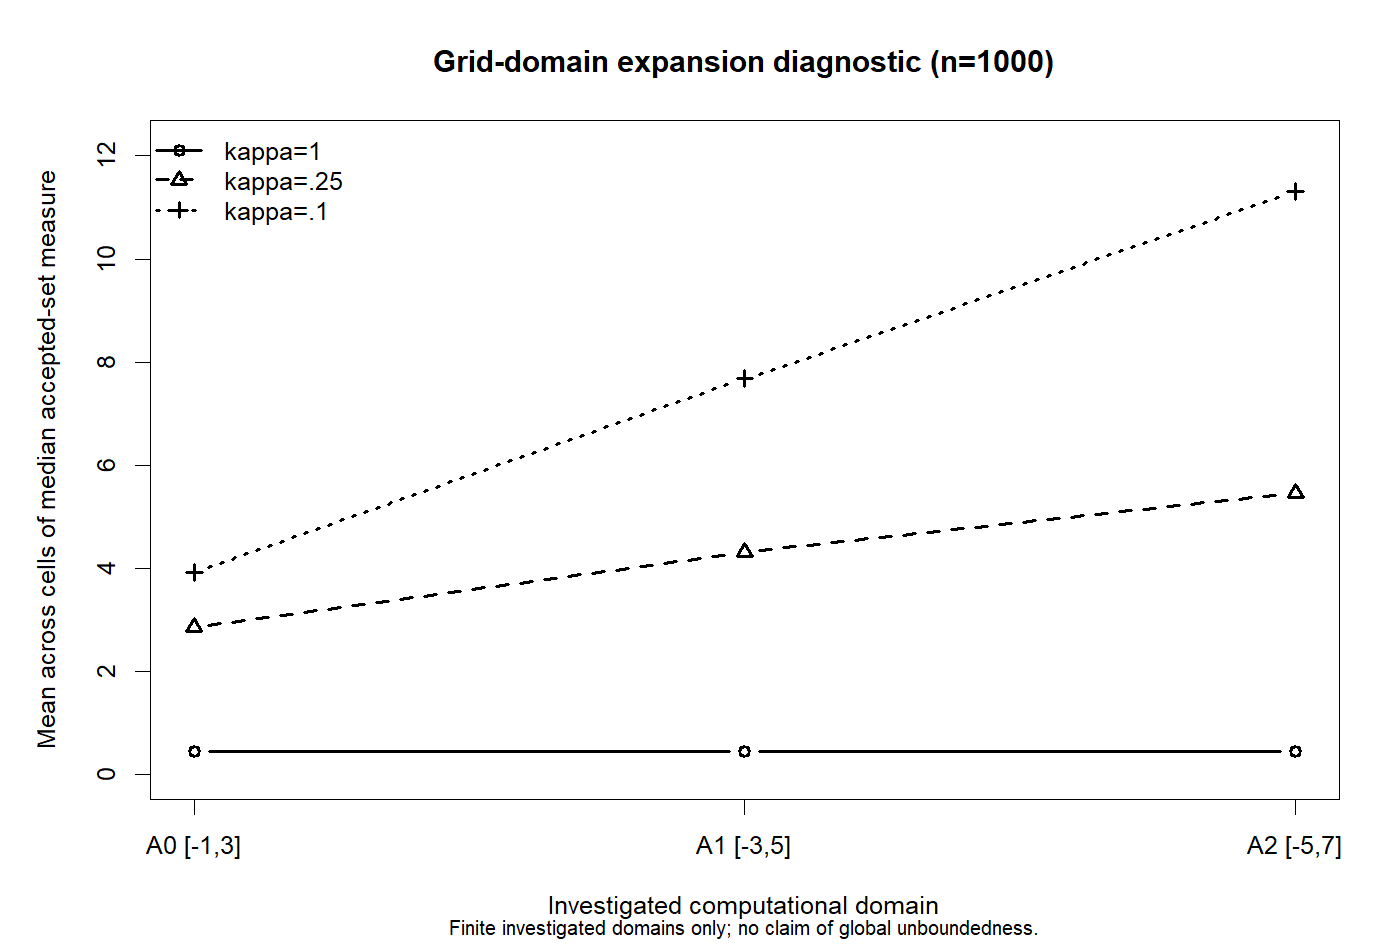
\includegraphics[width=0.72\textwidth]{figures/grid_domain_expansion.png}
  \caption{Sensitivity of the accepted set to expansion of the computational domain}
  \label{fig:grid-domain}
  \begin{figurenotes}[Note]
    Each plotted value is the mean across 15 estimator--quantile cells of the cell-specific median accepted-set measure for the stated $\kappa$ and domain. The investigated domains are $A_0=[-1,3]$, $A_1=[-3,5]$, and $A_2=[-5,7]$. The diagnostic records whether the accepted set stabilizes within these numerical domains; it does not establish global boundedness or unboundedness.
  \end{figurenotes}
\end{figure}

\FloatBarrier

Figure~\ref{fig:appendix_full_domain_acceptance} in Appendix~\ref{app:coverage-forensic-audit} complements these expansion diagnostics by reporting how often all candidates within the primary grid are accepted.
\Needspace{7\baselinedist}

\clearpage
\section{Derivation and Properties of the \texorpdfstring{$\kappa$}{kappa} Extension}
\label{app:kappa-derivation}
\setcounter{equation}{0}\setcounter{table}{0}\setcounter{figure}{0}
The extension changes assignment while retaining the baseline primitives in Section~\ref{sec:monte-carlo-design}. The excluded sum has variance two, $\epsilon_i$ has variance one, and $\operatorname{Cov}(u_i,\epsilon_i)=0.3$. Introduce independent $w_i\sim\mathcal N(0,1)$ and write
\begin{equation}
 d_i^*(\kappa)=\kappa(z_{1i}+z_{2i})+c(\kappa)w_i+\epsilon_i,
 \qquad \kappa\in[0,1].
 \label{eq:appendix-kappa-unknown}
\end{equation}
Independence eliminates all cross-covariances between index components. Preserving the baseline variance requires
\[
2\kappa^2+c(\kappa)^2+1=3,
\qquad c(\kappa)=\sqrt{2(1-\kappa^2)},\quad 0\le\kappa\le1.
\]
The nonnegative root is conventional; normal symmetry makes its sign distributionally immaterial. This coefficient is specific to the independent-noise construction. At $\kappa=0.50$, the signal variance is 0.5, replacement variance is 1.5, and $c(0.50)=\sqrt{1.5}\approx1.2247$. Calculations use the unrounded coefficient.
\begin{equation}
 \begin{aligned}
 d_i^*(\kappa)&=\kappa(z_{1i}+z_{2i})+\sqrt{2(1-\kappa^2)}\,w_i+\epsilon_i,\\
 D_i(\kappa)&=\Phi\!\left(d_i^*(\kappa)\right).
 \end{aligned}
 \label{eq:appendix-kappa-assignment}
\end{equation}
Normality gives $d_i^*(\kappa)\sim\mathcal N(0,3)$, where 3 denotes variance. Thus for $0<d<1$,
\begin{equation}
 \begin{aligned}
 \Pr\!\left[D_i(\kappa)\le d\right]
 &=\Pr\!\left[\Phi(d_i^*(\kappa))\le d\right]\\
 &=\Pr\!\left[d_i^*(\kappa)\le\Phi^{-1}(d)\right]\\
 &=\Phi\!\left(\frac{\Phi^{-1}(d)}{\sqrt{3}}\right).
 \end{aligned}
 \label{eq:appendix-treatment-cdf}
\end{equation}
The CDF is zero below zero and one above one. It is independent of $\kappa$, but is not Uniform$(0,1)$. Equal variance establishes this invariance because the index is normal, not for arbitrary distributions.

Write $Z_{ji}=z_{ji}+v_{ji}+C_{ji}$, where $C_{1i}=X_{2i}+X_{3i}+X_{4i}$ and $C_{2i}=X_{7i}+X_{8i}+X_{9i}+X_{10i}$. Independence yields
\[
\operatorname{Cov}(Z_{ji},d_i^*(\kappa))
=\kappa\operatorname{Cov}(z_{ji},z_{1i}+z_{2i})=\kappa,
\qquad j=1,2.
\]
The nonzero means of the control sums do not alter this covariance calculation. It concerns the latent index, and does not assert $\operatorname{Cov}(Z_{ji},D_i(\kappa))=\kappa$. Designed relevance is therefore distinct from a formal IVQR identification statistic.

Similarly, $\operatorname{Cov}(u_i,d_i^*(\kappa))=\operatorname{Cov}(u_i,\epsilon_i)=0.3$. Joint normality gives
\begin{equation}
 \begin{pmatrix}u_i\\d_i^*(\kappa)\end{pmatrix}
 \sim\mathcal{N}\!\left(
 \begin{pmatrix}0\\0\end{pmatrix},
 \begin{pmatrix}1&0.3\\0.3&3\end{pmatrix}\right).
 \label{eq:appendix-endogeneity-invariance}
\end{equation}
The invariant mean vector and covariance matrix establish invariance of the entire joint distribution, hence of $(u_i,\Phi(d_i^*(\kappa)))$. Covariance alone would not suffice without joint normality. Reusing primitive draws aids matched comparisons but is not needed for this distributional result; individual treatment realizations can differ across relevance settings.

At fixed $d>0$, $Y_i(d)=1+5\sum_{j=1}^7X_{ji}+d(1+u_i)$. Independence of $u_i$ and $X_i$ gives $Q_{Y_i(d)\mid X_i}(\tau)=1+5\sum_{j=1}^7X_{ji}+d[1+\Phi^{-1}(\tau)]$. The unchanged potential-outcome equation therefore preserves $\alpha_0(\tau)$. This is a structural quantile at fixed treatment, not an observational conditional quantile at realized endogenous treatment.

At $\kappa=1$ the replacement noise vanishes and the baseline is recovered. At the conceptual endpoint $\kappa=0$, $d_i^*(0)=\sqrt2w_i+\epsilon_i$, so the excluded primitive signal disappears. The weakest simulated setting retains signal variance $2(0.10)^2=0.02$. These endpoint statements establish properties of this construction, not global identification results for arbitrary IVQR models.

Table~\ref{tab:kappa-illustration} records the analytical variance allocation for all simulated settings.
\begin{table}[!htbp]
\caption{Variance allocation in the $\kappa$-extension.}
\label{tab:kappa-illustration}
\centering
\begin{tabular}{rrrrr}
\toprule
$\kappa$ & \shortstack{Coefficient\\$\sqrt{2(1-\kappa^2)}$} & \shortstack{Signal variance\\$2\kappa^2$} & \shortstack{Noise variance\\$2(1-\kappa^2)$} & \shortstack{Total index\\variance} \\
\midrule
1.00 & 0.0000 & 2.0000 & 0.0000 & 3.0000 \\
0.50 & 1.2247 & 0.5000 & 1.5000 & 3.0000 \\
0.25 & 1.3693 & 0.1250 & 1.8750 & 3.0000 \\
0.10 & 1.4071 & 0.0200 & 1.9800 & 3.0000 \\
\bottomrule
\end{tabular}
\begin{tablenotes}
Values are calculated directly from the construction, not simulated. The disturbance $\epsilon_i$ contributes the remaining variance of one in every row.
\end{tablenotes}
\end{table}

\FloatBarrier

\section{Coverage Audit and Inferential Informativeness}
\setcounter{equation}{0}\setcounter{table}{0}\setcounter{figure}{0}
\label{app:coverage-forensic-audit}

\subsection{Direct-at-Truth Coverage Audit}

Coverage is evaluated directly at the exact true structural effect $\alpha_0(\tau)$, independently of whether that value lies on the finite candidate grid. The forensic audit checked 60,000 direct truth evaluations: 500 replications for each of 120 sample-size, quantile, instrument-strength, and estimator cells.

Wilson 95\% Monte Carlo intervals exclude nominal $0.95$ coverage in 54 of the 120 cells. The audit finds no missing or nonfinite true-parameter $W$ statistics. The large coverage distortions reported in the main text are therefore neither plotting-grid artifacts nor consequences of missing-value handling. The frozen audit report and supporting diagnostics remain preserved in the repository. Wilson intervals are pointwise Monte Carlo uncertainty intervals, without simultaneous or multiplicity-adjusted significance claims. An individual rate's Monte Carlo standard error is not a standard error for a difference between correlated simulation results.

These checks rule out those numerical explanations for the reported coverage patterns. They do not establish correct theoretical specification, validate the asymptotic reference distribution for this DGP, or establish nominal finite-sample calibration.

\subsection{Coverage-Audit Summary}

Table~\ref{tab:coverage-audit-summary} summarizes the audit by estimator and sample size. Each row contains 20 quantile--$\kappa$ cells. Recalculation from integer acceptance counts reproduces 53 cells with an upper Wilson endpoint below 0.95 and one with a lower endpoint above 0.95, giving the reported total of 54. Comparisons use unrounded endpoints and the same 500-evaluation denominator in every cell.

\begin{table}[!ht]
\caption{Direct-at-truth coverage audit.}
\label{tab:coverage-audit-summary}
\centering
\begin{tabular}{lrrrrrrr}
\toprule
Estimator & $n$ & Cells & \shortstack{Coverage\\min.} & \shortstack{Coverage\\max.} & \shortstack{Upper\\$<0.95$} & \shortstack{Lower\\$>0.95$} & \shortstack{Missing/\\nonfinite} \\
\midrule
Oracle-GMM & 500 & 20 & 0.858 & 0.954 & 6 & 0 & 0 \\
Oracle-GMM & 1000 & 20 & 0.860 & 0.964 & 8 & 0 & 0 \\
Full-GMM & 500 & 20 & 0.442 & 0.962 & 9 & 0 & 0 \\
Full-GMM & 1000 & 20 & 0.502 & 0.962 & 12 & 0 & 0 \\
DML-IVQR & 500 & 20 & 0.658 & 0.976 & 8 & 1 & 0 \\
DML-IVQR & 1000 & 20 & 0.498 & 0.968 & 10 & 0 & 0 \\
\bottomrule
\end{tabular}
\begin{tablenotes}
Each row covers 20 quantile--$\kappa$ cells, with 500 direct-at-truth evaluations per cell. Coverage is reported as a proportion. The upper/lower columns count cells whose unrounded Wilson upper endpoint is below 0.95 or lower endpoint is above 0.95. Intervals use integer acceptance counts, the verified denominator, and the two-sided 95\% Wilson formula without continuity correction. They are pointwise Monte Carlo intervals, not simultaneous or multiple-testing-adjusted intervals; exclusion counts are descriptive audit summaries. Missing/nonfinite counts concern direct-at-truth $W$ evaluations (missing values are counted once).
\end{tablenotes}
\end{table}

\FloatBarrier

\subsection{Full-Domain Grid Acceptance}

The domain-expansion diagnostics in Appendix~\ref{app:numerical-domain-diagnostics} are complemented by Figure~\ref{fig:appendix_full_domain_acceptance}, which reports how often every evaluated point in the primary domain is accepted. Reading this frequency alongside coverage distinguishes retention of the true effect from the ability to exclude competing candidates within the maintained domain. Coverage near nominal can coexist with frequent acceptance of all primary-grid candidates: retaining the true value does not imply excluding alternatives.

The heatmap uses stored grid-profile evaluations, whereas coverage uses a separate evaluation directly at truth. These are distinct computations; in DML-IVQR, fresh pivotal draws can differ between them, so their acceptance events need not coincide even when truth is a grid point. Full-domain grid acceptance refers only to the 41 evaluated points in $A_0=[-1,3]$, not to acceptance of the real line or global unboundedness of an unrestricted confidence region.

\begin{figure}[!ht]
  \centering
  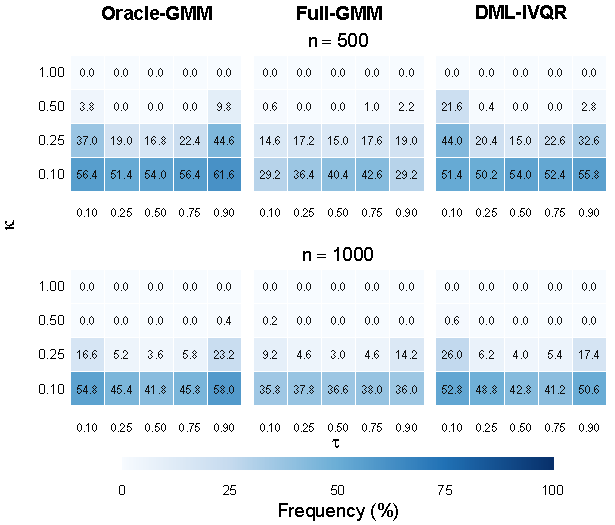
\includegraphics[width=0.72\textwidth]{figures/generated/full_domain_acceptance_heatmap.pdf}
  \caption{Full-domain grid acceptance frequencies.}
  \label{fig:appendix_full_domain_acceptance}
  \begin{figurenotes}
    Each cell reports the percentage of 500 complete replications accepting all 41 evaluated grid points in $A_0=[-1,3]$, with step size $h=0.1$. Panel columns identify estimators; panel rows show $n=500$ and $n=1000$. Within each panel, columns show quantiles $\tau$ and rows show relevance $\kappa$, declining from 1.00 to 0.10. Darker shading on the shared 0--100\% scale means more frequent full-domain grid acceptance. This event neither denotes acceptance of the entire real line nor establishes an unbounded unrestricted confidence region.
  \end{figurenotes}
\end{figure}

\FloatBarrier

\clearpage
\section{Reproducibility and Implementation Notes}
\label{app:reproducibility}
\setcounter{equation}{0}\setcounter{table}{0}\setcounter{figure}{0}
\subsection{Environment, records, and reproducibility limits}
The computational archive is the project repository \url{https://github.com/U-Olim/DML-IVQR_Master_Thesis}. This reference identifies the archived workflow; it is not a claim of bit-for-bit regeneration from a seed on arbitrary systems. Preserved source is in \path{simulation/}, \path{Empirical_work/}, and \path{example/}; extension wrappers and configuration are in \path{thesis_extension/src/} and \path{thesis_extension/config/extension_config.R}. The empirical freeze identifies commit \texttt{ac9a9ccad027cde05488abb633e66cc02f87cc46} (2 September 2026).

The canonical environment is R~3.4.3 (30 November 2017) on 64-bit Windows, using five workers. The captured attached packages are \texttt{doSNOW} 1.0.16, \texttt{snow} 0.4-2, \texttt{iterators} 1.0.8, \texttt{foreach} 1.4.3, \texttt{mvtnorm} 1.0-6, \texttt{hqreg} 1.4, \texttt{hdm} 0.2.0, \texttt{quantreg} 5.34, and \texttt{SparseM} 1.77. Environment session and library manifests are under \path{thesis_extension/environment/}. The main simulation uses seed 675; the grid diagnostic also uses seed 675, with saved primitives reloaded in Stage 2; calibration uses seed 20260813. Worker-specific RNG streams are not explicitly initialized in the preserved parallel DML procedure, so the parent seed alone does not establish exact regeneration of every penalty draw.

Frozen CSVs permit deterministic reporting without re-estimation. Input/output manifests in \path{thesis_extension/reporting/}, diagnostic provenance records, reporting consistency checks, and figure validation records connect the reported numbers to archived outputs. Historical manifests describe their archived presentation state and can retain former asset paths. The original figure check covered 480 plotted values; selected-figure validation separately covered 120 coverage values, 120 full-grid frequencies, and 168 median rejection probabilities. The coverage summary is reconstructed from integer direct-at-truth counts; the variance illustration is analytical. This editorial conversion does not rerun those historical validations or simulations.

\subsection{Penalty, density proxy, and residualization}
For each candidate, $b_0$ is the fitted outcome intercept and $b$ the slopes. In the preserved \texttt{rq.fit.lasso} augmented-observation implementation, the unscaled check-loss sum receives a penalty with factor $1/2$. The vector $\lambda^{rq}(a)$ is the supplied routine argument, including an intercept penalty. There is no post-Lasso refit. Let $s_k=(n^{-1}\sum_iX_{ik}^2)^{1/2}$; $U_{ir}$ are independent artificial Uniform$(0,1)$ draws, with $r=1,\ldots,1000$, and $\widehat Q_{0.9}$ is their empirical pivotal-statistic 90th percentile. Fresh draws are made on every penalty call. This is algorithmic randomness, not sample splitting.

In the following formulas, $\phi(e;\mu,\sigma)$ denotes a normal density parameterized by standard deviation. The proxy supplies $\widehat\sigma_\epsilon^2$ in that argument: the preserved R call is \texttt{dnorm(e, mean(e), var(e))}. It evaluates a fitted-normal density at residuals rather than estimating the theoretical conditional density at zero. The instrument penalty is $\mathcal P_{j,a}(\gamma_j)=\sum_k\lambda^\Gamma_{jk}(a)|\gamma_{jk}|$, using default iterative heteroskedastic loadings. Its ordinary intercept is unpenalized; no post-Lasso refit is performed.
\begin{equation}
    \begin{pmatrix}
        \widehat b_0(a)\\
        \widehat\beta(a)
    \end{pmatrix}
    =
    \operatorname*{arg\,min}_{b_0,b}
    \left\{
        \sum_{i=1}^{n}
        \rho_{\tau}\!\left(
            Y_i-D_i^{\prime}a-b_0-X_i^{\prime}b
        \right)
        +
        \frac{1}{2}\left[
            \lambda_0^{rq}(a)|b_0|
            +\sum_{k=1}^{p}\lambda_k^{rq}(a)|b_k|
        \right]
    \right\}.
    \label{eq:beta-hat-dml}
\end{equation}

\begin{equation}
    \begin{aligned}
        T_r
        &=
        \max_{1\leq k\leq p}
        \left|
            \frac{
                \sum_{i=1}^{n}X_{ik}
                \left[\tau-\mathbf{1}\{U_{ir}<\tau\}\right]
            }{
                s_k\sqrt{\tau(1-\tau)}
            }
        \right|,\\
        \lambda^{rq}(a)
        &=
        2\,\widehat Q_{0.9}\!\left(\{T_r\}_{r=1}^{1000}\right)
        \sqrt{\tau(1-\tau)}
        (1,s_1,\ldots,s_p)^{\prime}.
    \end{aligned}
    \label{eq:bc-pivotal-penalty}
\end{equation}

\begin{equation}
    \begin{aligned}
        \widehat{\epsilon}_i(a)
        &=
        Y_i-D_i^{\prime}a-\widehat b_0(a)
        -X_i^{\prime}\widehat{\beta}(a),\\
        \widehat{\mu}_{\epsilon}(a)
        &=\frac{1}{n}\sum_{i=1}^{n}\widehat{\epsilon}_i(a),\\
        \widehat f_i(a)
        &=
        \phi\!\left(
            \widehat{\epsilon}_i(a);
            \widehat{\mu}_{\epsilon}(a),
            \widehat{\sigma}_{\epsilon}^{2}(a)
        \right),
    \end{aligned}
    \label{eq:estimated-profile-residual}
\end{equation}

\begin{equation}
    \begin{pmatrix}
        \widehat r_{j0}(a)\\
        \widehat\Gamma_{\mathrm{imp},j}(a)
    \end{pmatrix}
    =
    \operatorname*{arg\,min}_{(r_{j0},\gamma_j)}
    \left\{
        \sum_{i=1}^{n}
        \left[
            \sqrt{\widehat f_i(a)}Z_{ji}
            -r_{j0}
            -\sqrt{\widehat f_i(a)}X_i^{\prime}\gamma_j
        \right]^2
        +\mathcal{P}_{j,a}(\gamma_j)
    \right\}.
    \label{eq:dml-residualization-implementation}
\end{equation}

\begin{equation}
    \begin{aligned}
        \widehat\Psi_{ji}(a)
        &=
        Z_{ji}-\widehat r_{j0}(a)-X_i^{\prime}\widehat\Gamma_{\mathrm{imp},j}(a),\\
        \widehat\Psi_i(a)
        &=
        Z_i-\widehat r_0(a)-\widehat\Gamma_{\mathrm{imp}}(a)X_i.
    \end{aligned}
    \label{eq:estimated-residualized-instrument}
\end{equation}

\begin{equation}
    \begin{pmatrix}
        \widehat b_{0,\mathrm{orc}}(a)\\
        \widehat\beta_{\mathrm{orc}}(a)
    \end{pmatrix}
    =
    \operatorname*{arg\,min}_{b_0,b}
    \sum_{i=1}^{n}
    \rho_{\tau}\!\left(
        Y_i-D_i^{\prime}a-b_0-X_{S_0,i}^{\prime}b
    \right).
    \label{eq:oracle-beta}
\end{equation}

\begin{equation}
    \begin{pmatrix}
        \widehat b_{0,\mathrm{full}}(a)\\
        \widehat\beta_{\mathrm{full}}(a)
    \end{pmatrix}
    =
    \operatorname*{arg\,min}_{b_0,b}
    \sum_{i=1}^{n}
    \rho_{\tau}\!\left(
        Y_i-D_i^{\prime}a-b_0-X_i^{\prime}b
    \right).
    \label{eq:full-beta}
\end{equation}

\begin{equation}
    \begin{aligned}
        \widehat M_e(a)
        &=\frac{1}{n}\sum_{i=1}^{n}
          Z_iX_{e,i}^{\prime}\widehat f_{e,i}(a),&
        \widehat J_e(a)
        &=\frac{1}{n}\sum_{i=1}^{n}
          X_{e,i}X_{e,i}^{\prime}\widehat f_{e,i}(a),\\
        \widehat\delta_e(a)
        &=\widehat M_e(a)\widehat J_e(a)^{-1},&
        \widehat\Psi_{e,i}(a)
        &=Z_i-\widehat\delta_e(a)X_{e,i}.
    \end{aligned}
    \label{eq:benchmark-residualization}
\end{equation}
The first five equations describe DML-IVQR. The last three describe Oracle-GMM and Full-GMM, with $S_0=\{1,\ldots,10\}$, $X_{\mathrm{orc},i}=X_{S_0,i}$, and $X_{\mathrm{full},i}=X_i$. Their quantile regressions include an intercept, but their matrix residualization includes no constant regressor. DML retains the ordinary intercept of a transformed regression and subtracts it from the original instrument without dividing by $\sqrt{\widehat f_i(a)}$. It is therefore not the exact sample counterpart of the ideal density-weighted intercept. All procedures use same-sample nuisance fits and scores; cross-fitting is absent. The comparison does not isolate regularization from these residualization differences.

\subsection{Score algebra and its conditions}
\label{app:score-algebra}
The ideal nuisance vector and derivative identities are retained below. They presume finite density-weighted moments and permissible differentiation, conditions not established for the simulation DGP's non-finite true residual density. They are not implementation-level assertions.
\begin{equation}
    \eta(a)
    =
    \begin{pmatrix}
        c(a)\\
        \beta(a)\\
        \operatorname{vec}\{\delta(a)\}
    \end{pmatrix},
    \qquad
    \eta_0
    =
    \eta\!\left(\alpha_0(\tau)\right)
    =
    \begin{pmatrix}
        c_0(\tau)\\
        \beta_0(\tau)\\
        \operatorname{vec}\{\delta(\alpha_0(\tau))\}
    \end{pmatrix}.
    \label{eq:profile-eta}
\end{equation}

\begin{equation}
    \operatorname{E}\!\left[
        \left\{
            \tau-\mathbf{1}\!\left[
                Y_i\leq D_i^{\prime}a+c(a)+X_i^{\prime}\beta(a)
            \right]
        \right\}\widetilde X_i
    \right]
    =0.
    \label{eq:profile-beta-moment}
\end{equation}

\begin{equation}
    \begin{aligned}
        M_0
        &=\operatorname{E}\!\left[
            Z_i\widetilde X_i^{\prime}
            f_{\epsilon_0}(0\mid X_i,Z_i)
        \right],\\
        J_0
        &=\operatorname{E}\!\left[
            \widetilde X_i\widetilde X_i^{\prime}
            f_{\epsilon_0}(0\mid X_i,Z_i)
        \right],\\
        \delta_0&=M_0J_0^{-1}.
    \end{aligned}
    \label{eq:orthogonality-MJ}
\end{equation}

\begin{equation}
    \begin{aligned}
        \left.
        \partial_{(c,\beta^{\prime})}
        \operatorname{E}\!\left[
            g_{\tau}\!\left(W_i;\alpha_0(\tau),\eta\right)
        \right]
        \right|_{\eta=\eta_0}
        &=-\operatorname{E}\!\left[
            (Z_i-\delta_0\widetilde X_i)\widetilde X_i^{\prime}
            f_{\epsilon_0}(0\mid X_i,Z_i)
        \right]\\
        &=-\left[M_0-\delta_0J_0\right]
        =0.
    \end{aligned}
    \label{eq:orthogonality-beta}
\end{equation}

\begin{equation}
    \left.
    \partial_{\delta_j}
    \operatorname{E}\!\left[
        g_{\tau,j}\!\left(W_i;\alpha_0(\tau),\eta\right)
    \right]
    \right|_{\eta=\eta_0}
    =-\operatorname{E}\!\left[
        \left\{
            \tau-\mathbf{1}\!\left[
                Y_i\leq D_i^{\prime}\alpha_0(\tau)
                +c_0(\tau)
                +X_i^{\prime}\beta_0(\tau)
            \right]
        \right\}\widetilde X_i^{\prime}
    \right]
    =0.
    \label{eq:orthogonality-delta}
\end{equation}
The first derivative cancels by $\delta_0=M_0J_0^{-1}$; the second cancels by the profiled quantile moment. Orthogonality concerns local nuisance sensitivity, and does not establish identification or finite-sample calibration.

\end{document}
